\documentclass[letterpaper,12pt]{article}
\usepackage{academicons}
\usepackage{xcolor}
\usepackage{graphicx}
\usepackage{physics}
\usepackage{algpseudocode}
\usepackage{listings}
\usepackage{comment} 


% @@@@@@@@@@@@@@@@@@@@@@@@@@@@@@@@@@@@@@@@@@@@@@@@@@@@@@@@@@@@>
% VALORES A MODIFICAR POR USTED:
% @@@@@@@@@@@@@@@@@@@@@@@@@@@@@@@@@@@@@@@@@@@@@@@@@@@@@@@@@@@@>

% NOTE: Leer nota en el README sobre la font.

\newcommand{\titulo}{Utilización de algoritmos cuánticos para mejorar rendimiento de simulaciones de nanoestructuras de una y dos dimensiones}
\newcommand{\ciudad}{Valpara\'iso} % e.g. Valparaíso
% TODO: Consultar el formato de los nombres:
\newcommand{\nombrealumno}{Javier Ignacio Norambuena Leiva}
\newcommand{\nombreprofesor}{Juan Manuel Florez Uribe}
\newcommand{\nombreprofesorcoguia}{Eric Suarez Morell}
\newcommand{\nombrecorreferente}{Raquel Pezoa Rivera}
% Mes y año del examen
\newcommand{\mesexamen}{Octubre}
\newcommand{\anioexamen}{2023}
% Dedicatoria y agradecimientos
\newcommand{\dedicatoria}{
¡Despertad, oh jóvenes de la nueva era! - Kenzaburo Oe
%Considerando lo importancia de este trabajo para los alumnos, este apartado es para que el autor entregue palabras personales para dedicar este documento. La extensión puede ser de máximo una hoja y se deben mantener este formato, tipo y tamaño de letra.
%Mi mente es una con el cielo y la tierra
}
\newcommand{\agradecimientos}{
%Considerando la importancia de este trabajo para los alumnos, este apartado se podrá incluir en el caso de que el autor desee agradecer a las personas que facilitaron alguna ayuda relevante en su trabajo para la realización de este documento. La extensión puede ser de máximo una hoja y se deben mantener este formato, tipo y tamaño de letra.
En primer lugar, me gustaría agradecer a mis padres, Juan Ricardo Villar y Paola Leiva Leviñanco por darme el apoyo y ánimos en este difícil proceso de desarrollo de la memoria. Agradecerles también de darme el espacio para poder concentrarme en el desarrollo y lograr graduarme a pesar de las dificultades.

Antes que cualquier otro agradecimiento, quiero agradecer a mi mejor amigo, Felipe Labra por su apoyo y compañía durante estos casi 17 años de amistad. Espero que esta amistad dure mucho más a pesar de que pronto nuestros caminos se separaran.

Quiero agradecerle a mi grupo de amigos que ya no están en esta universidad por todos los buenos momentos que pasamos, gracias Benjamín Montecinos, Paula Gallardo, Gabriel Osandón, Matías Reyes y Farid Funes por todo.

Quiero, además, agradecer al grupo de amigos que hice en mi estancia de en la universidad, los cuales me acompañaron en los mejores y peores momentos, gracias, Amanda Salinas, Valentina Espinoza, Camilo Castro, Emilio Oyanedel, Pedro Tobar, Nicolas Muñoz, Carlos Guerra y Catalina Silva.

Quiero agradecer a mis amigos civiles matemáticos que me adoptaron en su departamento, y una mención especial a Felipe Labra, Pedro Tobar, Nicolas Muñoz y Emilio Oyanedel que me ayudaron a no corromperme con laxidad de las demostraciones físicas y seguir el sendero del formalismo matemático.

Además, quiero agradecer a mi grupo de \textit{running}, que me ayudaron a no descuidar mi salud física, gracias, Amanda Salinas y Valentina Espinoza por tantas risas y competiciones en las que participamos.

Luego quiero agradecer al profesor Juan Manuel, al profesor Eric Suarez y a todo el grupo de simulaciones del departamento de física por darme la oportunidad de trabajar en el área que me gusta, la de la computación cuántica. No saben cómo les agradezco su ayuda, la dedicación y la amabilidad de ayudar a alguien ajeno a la física a entrar en el mundo de desarrollar métodos computacionales y entender la física detrás de los resultados. 

No me es posible colocar todos los nombres que me gustaría pero, quiero que si esas personas leen este escrito, sepan que tienen un lugar en mi corazón.


}
\newcommand{\resumen}{
La computación cuántica se ha vuelto un tema de interés en países del primer mundo debido al desarrollo de máquinas de sobre 100 \textit{qubits}, es por ello por lo que, es importante involucrarse en esta área por las proyecciones en el futuro próximo y las posibilidades que ofrece el uso de máquinas cuánticas frente a las tradicionales.

Este trabajo constituye una primera versión de un esquema de flujo de trabajo, además de un análisis en torno al uso de recursos de las aplicaciones de métodos cuánticos para el estudio de sistemas físicos de la materia condensada y quimica cuantica, en el contexto de la física computacional. Estas técnicas se pusieron a prueba en diferentes estructuras para generar un constaste con las técnicas más famosas en el área.

%El resumen y las palabras clave no deben superar la mitad de la página, donde debe precisarse brevemente: 1) lo que el autor ha hecho, 2) cómo lo hizo (sólo si es importante detallarlo), 3) los resultados principales, 4) la relevancia de los resultados. El resumen es una representación abreviada, pero comprensiva de la memoria y debe informar sobre el objetivo, la metodología y los resultados del trabajo realizado.
}
\newcommand{\resumeningles}{
\textit{The quantum computing become one of the mayor topic of interest in the development countries, this is because of the development of quantum machine with over a 100 qubits, for near-term projections and the possibilities that offer the quantum machine are the major reason to start working in this area}.

\textit{This work constitutes the first attempt to construct a workflow and perform an analysis of the resources usage of the quantum method in the study of condensed matter physics's systems and quantum chemistry systems in the context of computational physics. This methods were put in constract with other techniques in different structures}.

%Corresponde a la traducción al idioma inglés del Resumen anterior. Sujeto a la misma regla de extensión del Resumen.
}
\newcommand{\palabrasclave}{
Física computacional, Computación cuántica, Física del estado solido, Química cuántica, Análisis de rendimiento.
}
\newcommand{\palabrasclaveingles}{
\textit{Computational physics, Quantum computing, Solid state physics, Quantum chemistry, Performance analysis}.
}
% @@@@@@@@@@@@@@@@@@@@@@@@@@@@@@@@@@@@@@@@@@@@@@@@@@@@@@@@@@@@>

% Paquete para importar imágenes
\usepackage{graphicx}
% Directorio de las imágenes
\graphicspath{ {figures/} }

% Idioma y fuentes
\usepackage[spanish,es-tabla]{babel}
\usepackage[T1]{fontenc}

\usepackage{fontspec}
% Los siguientes comandos fueron sugeridos por @anibalbastiass (ver issue#5)
% para contar con Carlito en cursiva y negrita.
\setmainfont{Carlito}[BoldFont={* Bold}]
\setmainfont{Carlito}[ItalicFont={* Italic}]

% Paquete para definir cualquier tamaño de font
\usepackage{anyfontsize}

% Settear font
\setmainfont{Carlito}

% Tamaño de la página y márgenes
\usepackage[letterpaper,top=2.5cm,bottom=3cm,left=3cm,right=3cm,marginparwidth=1.75cm]{geometry}

% Determinar interlineado:
\renewcommand{\baselinestretch}{1.0}

% Eliminar sangrías:
\setlength{\parindent}{0cm}

% Paquete para definir los formatos de los títulos
\usepackage[explicit]{titlesec}

\titleformat{name=\section}[block]{\fontsize{16}{24}\selectfont\bfseries}{}{0pt}{#1}
\titleformat{name=\section,numberless}[block]{\fontsize{16}{24}\selectfont\bfseries}{}{0pt}{#1}
\titlespacing*{name=\section}{0pt}{0pt}{0.5cm}
\titlespacing*{name=\section,numberless}{0pt}{0pt}{0.5cm}

% Separación entre parrafos
\setlength{\parskip}{0.4cm}

% Paquetes de utilidad general
\usepackage{amsmath}
\usepackage{graphicx}
\usepackage{float}
\usepackage[colorlinks=true, allcolors=blue]{hyperref}

% Formato de las tablas de contenido
% \usepackage[tocflat]{tocstyle}
\usepackage{tocstyle}
\usetocstyle{allwithdot}

% Para obtener el número de la última página
\usepackage{lastpage}

% Header y footer
\usepackage{fancyhdr}
\fancypagestyle{portada}{
    \lhead{}
    \chead{}
    \rhead{}
    \lfoot{}
    \cfoot{\fontsize{10}{12}\selectfont \thepage}
    \rfoot{}
    \renewcommand{\headrulewidth}{0pt}
}
\fancypagestyle{intermedio}{
    \lhead{}
    \chead{\fontsize{10}{12}\selectfont\MakeUppercase{\titulo}}
    \rhead{}
    \lfoot{}
    \cfoot{\fontsize{10}{12}\selectfont Página \textbf{\thepage}\ de \textbf{\pageref{LastPage}}}
    \rfoot{}
    \renewcommand{\headrulewidth}{1pt}
}

% Comandos para secciones
\newcommand{\secnumbersection}[1]{
\addtocounter{section}{1}
\phantomsection
\section*{CAPÍTULO \thesection \texorpdfstring{\\}\ #1}
\addcontentsline{toc}{section}{CAPÍTULO \thesection : #1}
\setcounter{subsection}{0}
}
\newcommand{\secnumberlesssection}[1]{
\section*{#1}
\phantomsection
\addcontentsline{toc}{section}{#1}
\setcounter{subsection}{0}
}

% Nombres
\addto\captionsspanish{\renewcommand{\contentsname}{ÍNDICE DE CONTENIDOS}}
\addto\captionsspanish{\renewcommand{\listfigurename}{ÍNDICE DE FIGURAS}}
\addto\captionsspanish{\renewcommand{\listtablename}{ÍNDICE DE TABLAS}}
\makeatletter
\renewenvironment{thebibliography}[1]
     {\secnumberlesssection{REFERENCIAS BIBLIOGRÁFICAS}
      \@mkboth{\MakeUppercase\bibname}{\MakeUppercase\bibname}%
      \list{\@biblabel{\@arabic\c@enumiv}}%
           {\settowidth\labelwidth{\@biblabel{#1}}%
            \leftmargin\labelwidth
            \advance\leftmargin\labelsep
            \@openbib@code
            \usecounter{enumiv}%
            \let\p@enumiv\@empty
            \renewcommand\theenumiv{\@arabic\c@enumiv}}%
      \sloppy
      \clubpenalty4000
      \@clubpenalty \clubpenalty
      \widowpenalty4000%
      \sfcode`\.\@m}
     {\def\@noitemerr
       {\@latex@warning{Empty `thebibliography' environment}}%
      \endlist}
\makeatother

% Personalizar Tabla de Contenidos

\usepackage{tocloft}
\renewcommand{\cftsecfont}{\fontsize{12}{14}\selectfont\fontspec{Carlito}}
\renewcommand{\cftsubsecfont}{\fontsize{12}{14}\selectfont\fontspec{Carlito}}
\renewcommand{\cftsubsubsecfont}{\fontsize{12}{14}\selectfont\fontspec{Carlito}}

\renewcommand\cftfigfont{\fontsize{12}{14}\selectfont\fontspec{Carlito}}

% Links sin color
\usepackage{hyperref}
\hypersetup{colorlinks = false}

% Comando para secciónes sin enumeración
% (sugerido por @anibalbastiass https://github.com/autopawn/tex-thesis-template/issues/5#issuecomment-916106128)
\newcommand{\secnumberlesssubsection}[1]{
\subsection*{#1}
\phantomsection
\addcontentsline{toc}{subsection}{#1}
\setcounter{subsection}{0}
}
% Forma de uso:
% \secnumberlesssubsection{"Sub seccion sin enumeración"}

% @@@@@@@@@@@@@@@@@@@@@@@@@@@@@@@@@@@@@@@@@@@@@@@@@@@@@@@@@@@@>
\begin{document}
\sloppy % Para evitar que referencias se escapen de los márgenes.

\pagestyle{portada}
\pagenumbering{roman}
% NOTE: Este archivo contiene la portada, la dedicatoria, los agradecimientos y el resumen.
% __NO ES NECESARIO MODIFICAR ESTE ARCHIVO__, esas se modifican con los comandos que aparecen en main.tex
%@@@@@@@@@@@@@@@@@@@@@@@@@@@@@@@@@@@@@@@@@@@@@@@@@@@@@@@@@@@@@@
\begin{titlepage}
\begin{center}
\noindent
{\fontsize{18}{22}\selectfont UNIVERSIDAD TÉCNICA FEDERICO SANTA MARÍA \\}
{\fontsize{16}{19}\selectfont DEPARTAMENTO DE INFORMÁTICA \\}
{\fontsize{16}{19}\selectfont \MakeUppercase{\ciudad}\ - CHILE \\}
\vspace{1.5cm}

\includegraphics[width=4.41cm,height=3.34cm]{logo/logo.jpg} \\
\vspace{1.5cm}
{\fontsize{20}{24}\selectfont ``\MakeUppercase{\titulo}'' \\}
\vfill
{\fontsize{16}{19}\selectfont \MakeUppercase{\nombrealumno} \\}
\vfill
{\fontsize{16}{19}\selectfont MEMORIA PARA OPTAR AL TÍTULO DE \\}
{\fontsize{16}{19}\selectfont INGENIERO CIVIL EN INFORMÁTICA \\}
\vspace{1.5cm}
{\fontsize{14}{17}\selectfont Profesor Guía: \nombreprofesor \\}
{\fontsize{14}{17}\selectfont Profesor Co-guía: \nombreprofesorcoguia \\}
{\fontsize{14}{17}\selectfont Profesora Correferente: \nombrecorreferente \\}
\vspace{2.5cm}
{\fontsize{14}{17}\selectfont \mesexamen\ - \anioexamen \\}
\end{center}
\end{titlepage}

%@@@@@@@@@@@@@@@@@@@@@@@@@@@@@@@@@@@@@@@@@@@@@@@@@@@@@@@@@@@@@@
\newpage
\setcounter{page}{2}
\
\vfill
\vfill
\begin{flushright}
\noindent {\fontsize{16}{19}\selectfont \textbf{DEDICATORIA} \\}
\end{flushright}
\begin{flushright}
\noindent \dedicatoria 
\end{flushright}
\vfill
%@@@@@@@@@@@@@@@@@@@@@@@@@@@@@@@@@@@@@@@@@@@@@@@@@@@@@@@@@@@@@@
\newpage
\begin{center}
\noindent {\fontsize{16}{19}\selectfont \textbf{AGRADECIMIENTOS} \\}
\end{center}
\noindent \agradecimientos
\vfill
%@@@@@@@@@@@@@@@@@@@@@@@@@@@@@@@@@@@@@@@@@@@@@@@@@@@@@@@@@@@@@@
\newpage
\secnumberlesssection{RESUMEN}
\vspace{0.3cm}
\noindent \textbf{Resumen---}\resumen \ \\
\vspace{0.3cm} \\
\noindent \textbf{Palabras Clave---}\palabrasclave \ \\
% @@@@@
\vspace{1.2cm} \\
% @@@@@
%\noindent {\fontsize{16}{19}\selectfont \textbf{ABSTRACT}}
%\vspace{1.2cm} \\
\secnumberlesssection{ABSTRACT}
\vspace{0.3cm}
\noindent \textbf{\emph{Abstract}---}\resumeningles \ \\
\vspace{0.3cm} \\
\noindent \textbf{\emph{Keywords}---}\palabrasclaveingles \ \\
%@@@@@@@@@@@@@@@@@@@@@@@@@@@@@@@@@@@@@@@@@@@@@@@@@@@@@@@@@@@@@@


\newpage
\secnumberlesssection{GLOSARIO}

%Aquí se deben colocar las siglas mencionadas en el trabajo y su explicación, por orden alfabético. Por ejemplo: \\

{\setlength{\parskip}{0cm} % Para evitar saltar entre cada elemento nombrado.
%Colocar aquí siglas:

a.u: \textit{Atomic Units}

CCCBD : \textit{Computational Chemistry Comparison and Benchmark DataBase}

CPU : \textit{Central Processing Unit}

DMRG: \textit{Density matrix renormalization group}

eV: Electronvoltio

GPU: \textit{graphics processing unit}

HE: \textit{Hardware efficient}

K: Kelvin

k-UpCCGSD: \textit{k-Unitary pair Coupled Cluster Generalized Singles and Doubles} 

mb: Megabytes

MPS: \textit{Matrix product states}

MPO: \textit{Matrix product operators}

NISQ: \textit{Noisy intermediate-scale quantum}
%SMM: Single molecular magnets

VQE: \textit{Variational quantum deflation}

VQE: \textit{Variational quantum eigensolver}

VQT: \textit{Variational quantum thermalizer}

UCCSG: \textit{Unitary Coupled Cluster Single Doubles}


}



%Índice de contenidos:
\newpage
\thispagestyle{portada}
\tableofcontents

%Índice de figuras:
\newpage
\thispagestyle{portada}
\phantomsection
\addcontentsline{toc}{section}{ÍNDICE DE FIGURAS}
\listoffigures
\phantomsection
\addcontentsline{toc}{section}{ÍNDICE DE TABLAS}
\listoftables

\newpage
\pagestyle{intermedio}
\pagenumbering{arabic}
\secnumberlesssection{INTRODUCCIÓN}

Dentro de la física computacional, uno de los mayores desafíos es el poder desarrollar métodos computacionales que puedan simular los fenómenos físicos de la manera más precisa posible. Esto suele derivar en un problema de \textit{trade-off}, donde uno tiene que sacrificar grados de libertad por viabilidad computacional.

En las últimas décadas, se ha experimentado un desarrollo de múltiples métodos que permiten que este \textit{trade-off} no sacrifique la calidad de los resultados de las simulaciones y el tipo de sistemas que se pueden resolver. En los últimos años, se ha visto un aumento en el uso de redes tensoriales \cite{Hauschild_2018} \cite{SCHOLLWOCK201196} para el estudio de sistemas físicos \cite{tensor1} \cite{tensor2} y de \textit{machine learning} (\textit{deep learning}) para la estimación de características \cite{MachineLearning1J}\cite{MachineLearning2}.

Frente a este panorama es que otro método ha surgido como solución, el cual trae un nuevo paradigma, para llevar a cabo simulaciones, que es la computación cuántica. Durante los últimos años, ha adquirido gran relevancia debido a los progresos de grandes compañías como IBM y Google, quienes han desarrollado procesadores de 50 a 200 \textit{qubits} (\textit{sycamore} e \textit{IBM eagle}) \cite{Stanisic2022} \cite{Powers2023}(Esto ha fomentado diversas nuevas investigaciones \cite{Stanisic2022} \cite{Powers2023} de diverso carácter que muestran el potencial de la computación cuántica.

En el presente trabajo se propone y estudia un flujo de trabajo/cálculo para la implementación y utilización de algoritmos cuánticos para el estudio de diversos modelos de la física del estado sólido, la materia condensada y la química. Para ello, se utilizan librerías especializadas en el trabajo de circuitos cuánticos, además de una revisión del estado actual del arte para trabajar con un conjunto de hiperparámetros adecuados para cada modelo. El algoritmo central en el desarrollo de la memoria es el método VQE (junto a un par de variaciones), el cual es puesto a prueba en diferentes modelos cuyos estados tienen diferentes niveles de correlaciones (haciendo del cálculo más o menos complejo), con el objetivo de mostrar su viabilidad y potencial.

El escrito se divide en cinco capítulos con un anexo. Los primeros dos capítulos consisten en la presentación del problema y conceptos clave para entender el desarrollo realizado (marco conceptual). En el tercer capítulo se presenta la solución propuesta con los límites y supuestos considerados en el desarrollo. El cuarto capítulo se divide en cuatro subcapítulos, en cada uno se analizan características distintas (las cuales requieren metodologías distintas que son presentadas antes de los resultados). Finalmente, en el capítulo cinco se presentan las conclusiones en cuatro subcapítulos, el primero, son unas palabras acerca de los resultados obtenidos, después, un análisis sobre los objetivos y los últimos son el trabajo futuro y las palabras finales del autor. En el anexo se presenta el enlace al repositorio del proyecto junto a los datos obtenidos.


\newpage
\secnumbersection{DEFINICIÓN DEL PROBLEMA}

\subsection{Contexto del problema}

La física computacional es un área multidisciplinaria cuyo objetivo es el desarrollo de modelos que permitan caracterizar fenómenos físicos derivados de las interacciones entre partículas, así como, crear métodos computacionales que nos permitan estudiar y generar predicciones del comportamiento de estas. Para el presente proyecto, únicamente consideraremos las áreas de la materia condensada, la física del estado sólido y la química.

Uno de los desafíos que se presentan en la investigación de estas estructuras radica en la cantidad de niveles de libertad que están pueden tener. Considerando que la materia está compuesta por muchas partículas (electrones, protones y neutrones), el tener en cuenta todas las posibles interacciones se vuelve una tarea muy difícil. Esto puede observarse en la siguiente expresión, que engloba las interacciones electrostáticas no relativistas entre partículas.

\begin{equation*}
    \mathcal{H} = -\sum_{i=!}^{N}\frac{1}{2}\nabla_i^2 - \sum_{A = 1}^{M} \frac{1}{2M_A}\nabla_A^{2} -\sum_{i=1}^{N}\sum_{A = 1}^{M} \frac{Z_A}{r_{iA}} + \sum_{i=1}^{N}\sum_{j>i}^{N} \frac{1}{r_{ij}}  + \sum_{A=1}^{M}\sum_{B>A}^{M} \frac{Z_AZ_B}{R_{AB}}
\end{equation*}

Frente a este dilema es que, teóricamente, se han propuesto diferentes aproximaciones que, bajo ciertos supuestos, permiten despreciar términos y tratar otros como valores constantes, reduciendo así las expresiones y los grados de libertad.

Una de las aproximaciones más famosa es la aproximación de Born-Oppenheimer\cite{BornOppenheimer}. Dado el modelo molecular de interacciones electrostáticas, si tomamos en cuenta la diferencia entre la energía cinética de los electrones frente al núcleo, es posible reducir la expresión original a la siguiente:

\begin{equation*}
    \mathcal{H}_{elec} = -\sum_{i=!}^{N}\frac{1}{2}\nabla_i^2  -\sum_{i=1}^{N}\sum_{A = 1}^{M} \frac{Z_A}{r_{iA}} + \sum_{i=1}^{N}\sum_{j>i}^{N} \frac{1}{r_{ij}}
\end{equation*}

El problema de este tipo de aproximaciones es que, a pesar de que se reduce el número de interacciones y grados de libertad, a medida que se tengan estructuras más complejas, el número de partículas sigue siendo muy grande (seguimos teniendo un problema de muchos cuerpos). De estas aproximaciones teóricas es que surgen los diversos hamiltonianos, los cuales son modelos que se enfocan en interacciones concretas, todos estos modelos son construidos en representaciones matriciales. Lamentablemente, estos siguen teniendo problemas de crecimiento a medida que se aumenta el número de partículas.

Para ejemplificar esto, consideremos un sistema de espines (el cual solo toma en cuenta las interacciones de los espines), que son representados como sumas de productos tensoriales de matrices cuadradas (matrices de Pauli), que tienen dimensión $(2S+1)^{2n}$ (siendo $n$ el tamaño del sistema y $S$ el espín). En la figura \ref{fig:1000} se puede apreciar los requerimientos de memoria RAM para mantener ese tipo de hamiltoniano en memoria, teniendo en cuenta diversos espines.


\begin{figure}[H]
\centering
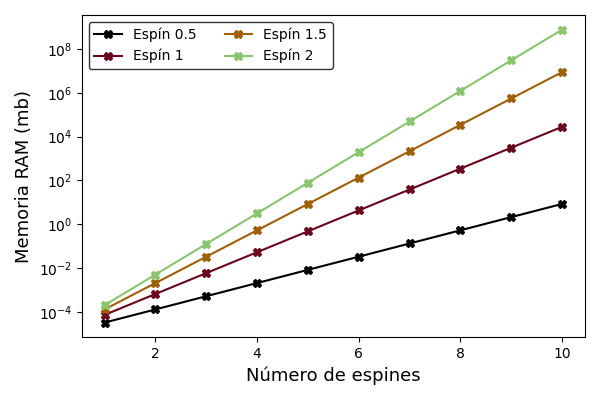
\includegraphics[width=0.7\textwidth]{figures/S1/matriz.png}
\caption{\label{fig:1000} Requerimientos de memoria RAM él para modelo de espines. Fuente: Elaboración propia}
\end{figure}

El segundo problema es que hay que encontrar los elementos necesarios para poder realizar estudios y proyecciones de los efectos derivados de interacciones externas sobre el hamiltoniano. Por ejemplo, para realizar estudios que consideren los efectos de la temperatura, por la descripción matemática del operador de densidad, es necesario tener todos los valores y vectores propios del hamiltoniano. Para hacer esto, es necesario diagonalizar la matriz asociada, lo cual es una tarea computacionalmente costosa cuando el hamiltoniano considera muchas partículas. 


Esta situación presenta un gran obstáculo al momento de realizar investigaciones sobre el comportamiento de la materia, por un lado, si uno desea estudiar sistemas de gran dimensionalidad (muchos cuerpos), se está limitado a trabajar con tipos de hamiltonianos muy concretos que ofrecen una escalabilidad (tamaño de la matriz del modelo) razonable para llevar a cabo una diagonalización exacta, el problema con esto, es que este tipo de hamiltonianos utilizan muchos supuestos, por lo que se puede poner en duda los comportamientos que se pueden derivar de este. Por el otro lado, uno puede realizar estudios exhaustivos (estudios termodinámicos) sobre sistemas de pocos cuerpos, pero lamentablemente, no siempre se puede extrapolar el comportamiento de pocos cuerpos a muchos cuerpos.


\subsection{Estado actual del problema}
Debido a la popularidad de métodos basados en \textit{Density functional theory}, teoría de Hartree-Fock y técnicas basadas en primeros principios, en las últimas décadas se han propuesto diferentes representaciones para tener un uso de recursos más eficiente, además de, crear nuevos métodos con una mejor escalabilidad. Entre ellos, se encuentra la representación MPS/MPO junto al método variacional DRMG que utiliza el concepto de redes tensoriales para representar los sistemas y calcular su estado de mínima energía. Por otro lado, se tienen las aplicaciones de redes neuronales para generar estimadores utilizando resultados, de métodos de \textit{Density functional theory}\cite{Yin2021}, con un bajo error. Las técnicas y métodos mencionados anteriormente corresponden a un paradigma que denominaremos métodos clásicos (que engloban desde métodos exactos hasta métodos variacionales).

En los últimos años, se ha popularizado el uso de computadores cuánticos para realizar simulaciones de sistemas físicos. La computación cuántica no había adquirido esta popularidad porque no existían máquinas cuánticas reales. Desde hace un par de años, Google e IBM anunciaron al público las primeras máquinas cuánticas de pocos \textit{qubits}, las cuales abrieron nuevas posibilidades de aplicaciones y desarrollo en el campo. 

Estas máquinas permiten escapar de la representación matricial, ya que, se trabaja directamente con las funciones de onda que se almacenan en cada \textit{qubits}, por otro lado, se ha demostrado que los algoritmos que se ejecutan en estas máquinas tienen un rendimiento igual o mejor que los algoritmos clásicos (ejemplos de esto es el algoritmo de factorización de números primos de Shor, el algoritmo de Grover entre otros).

Frente a este nuevo paradigma y con los pronósticos de capacidad de las nuevas máquinas, es menester empezar a trabajar en esta área, ya que, al ser un área tan reciente, aún existen muchas aristas en las cuales trabajar (aplicaciones, desarrollo de nuevos métodos, etc.).


\subsection{Objetivos de la solución}
\subsubsection{Objetivo general}
El objetivo general del proyecto es ''Analizar el uso de algoritmos variacionales cuánticos en las simulaciones de estructuras físicas en el contexto de química cuántica y materia condensada''. Este análisis tiene por objetivo visualizar el uso de recursos (de memoria y tiempo) además de contrastar las soluciones obtenidas con los valores exactos.

\subsubsection{Objetivos específicos}
\begin{enumerate}
\item Realizar un estudio que muestre los requerimientos de almacenamiento de los modelos de tipo Fermi-Hubbard, \textit{tight binding}, Heisenberg y estructuras moleculares.
\item Realizar un \textit{benchmark} que contraste los tiempos de ejecución y el error absoluto asociado a la solución obtenida, para el problema de valores y vectores propios, de un algoritmo clásico-exacto, clásico-variacional y variacional cuántico, considerando los modelos expuestos en el punto 1
\item Proponer un diagrama de flujo de trabajo para la utilización algoritmo cuántico, que permita ser generalizado a una amplia gama de hamiltonianos y sistemas de baja dimensión, utilizando rutinas de código abierto y de elaboración propia.
\item Ilustrar la efectividad del diagrama propuesto al aplicarlo en sistemas físicos de baja dimensionalidad.
\end{enumerate}

\subsubsection{Alcance}
Durante el desarrollo del proyecto, se decidió acotarlo en los siguientes aspectos:
\begin{enumerate}
    \item Los parámetros de los modelos se acotaron a regiones y estructuras específicas para limitar el número de posibles combinaciones con los hiperparámetros del \textit{ansatz} y del optimizador (mayor detalle en el capítulo 3).
    \item Por los costos monetarios de uso, se descartó el uso de máquinas cuánticas reales.
\end{enumerate}


\newpage
\secnumbersection{MARCO CONCEPTUAL}

\subsection{\textit{Qubits}, compuertas y algoritmos cuánticos}

Un \textit{qubit} puede ser entendido desde la perspectiva de un sistema físico que tiene un comportamiento de sistema de dos niveles (entre otras muchas características), pero también se puede entender desde una perspectiva más matemática. Para esta memoria, se tomará esta segunda perspectiva (debido a que se buscan aplicaciones de alto nivel), para ello se parte de la premisa de que no importa de que está hecho el \textit{qubit}, sino que, nos importa la descripción y las propiedades matemáticas asociadas a este objeto.

\subsubsection{Que es un \textit{qubit}}
Un \textit{qubit} al igual que un bit, corresponde a un estado, pero a diferencia de este último (que solo puede estar en $0$ o $1$), los \textit{qubits} pueden estar en una infinidad de estados gracias a la combinación lineal de los estados basales. 
\begin{equation*}
    \ket{\psi} = \alpha \ket{0} + \beta \ket{1}
\end{equation*}
Donde $\alpha$ y $\beta$ corresponden a números complejos que cumplen con $|\alpha|^2 + |\beta|^2 = 1$. Esto es posible, ya que, los \textit{qubits} son objetos que se rigen por las leyes de la mecánica cuántica, las cuales permiten construir estados como combinaciones lineales mientras estos no sean observados, en el momento de que esto ocurra el estado colapsa a uno de los que componen la combinación lineal y este objeto cuántico pasa a comportarse como uno clásico. En la literatura, es común encontrar a los \textit{qubits} representados como esferas \ref{fig:EsferaBloch}, siendo los estados, puntos del manto de la misma. Esta representación se conoce como la esfera de Bloch.

\begin{figure}[H]
\centering
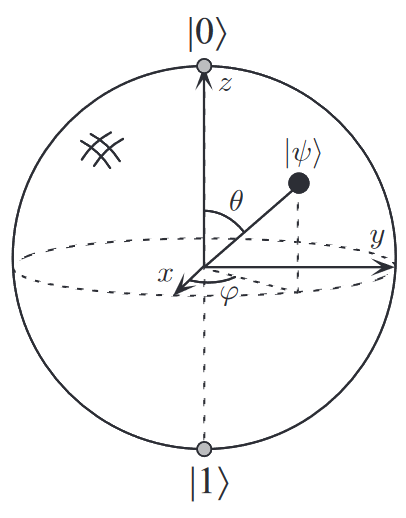
\includegraphics[width=0.3\textwidth]{figures/S2/ESFERABLOCH.png}
\caption{\label{fig:EsferaBloch} Representación de un \textit{qubit} en la esfera de Bloch. Fuente: \cite{nielsen_chuang_2010}}
\end{figure}

Para construir un estado de un sistema de muchos \textit{qubits} (independientes entre sí), lo que se realiza es aplicar el producto Kronecker (producto tensorial) entre cada uno de los estados, lo que crea un vector de tamaño $2^n$ (siendo $n$ el número de \textit{qubits}). La notación de este producto es equivalente a la de muchos bits $\ket{\psi_1\psi_2 ... \psi_n}$ (los $\psi_i$ corresponde a los estados de cada \textit{qubit}).

\subsubsection{Como operar con un \textit{qubit}}
Las acciones que se aplican a los \textit{qubits} corresponden a la aplicación de operadores, estos operadores en la literatura son conocidos como compuertas. Una de las ideas claves es el concepto de la reversibilidad de las operaciones, es decir, que después de aplicar una cierta secuencia de operaciones a un estado inicial, podamos ser capaces de volver al estado original, para lograr esto, se pide que las compuertas sean unitarias, esto quiere decir que, siendo $U$ una compuerta, tiene que verificar $UU^{\dag}=U^{\dag}U=I$.

En la literatura, es común que las compuertas sean presentadas en dos grupos, las compuertas de un solo \textit{qubit} y las de muchos \textit{qubits}. Las compuertas de un solo \textit{qubit} se interpretan como operadores de rotación (teniendo en mente la esfera de Bloch), lo que hacen estos operadores es mover el estado por el manto de la esfera. A continuación, se entrega la descripción matricial junto a una interpretación rotacional de las matrices de un solo \textit{qubits} más famosas.

\begin{enumerate}
 \item Compuerta X: Esta compuerta lo que realiza es un intercambio entre la probabilidad de los estados, es decir, aplica una rotación de 180 grados respecto al eje X.
    \begin{equation*}
    X = 
        \begin{pmatrix}
        0 & 1\\
        1 & 0
        \end{pmatrix}
    \end{equation*} 
    \item Compuerta Y: Puede ser entendida como una rotación respecto al eje Y por 180 grados.
    \begin{equation*}
    Y = 
        \begin{pmatrix}
        0 & -i\\
        i & 0
        \end{pmatrix}
    \end{equation*} 
    \item Compuerta Z: Esta compuerta realiza un cambio de signo de la componente $\ket{1}$. Al igual que las compuertas anteriores, también es una rotación respecto al eje Z por 180 grados.
    \begin{equation*}
    Z = 
        \begin{pmatrix}
        1 & 0\\
        0 & -1
        \end{pmatrix}
    \end{equation*}
    \item Compuerta I: La compuerta identidad no realiza nada, deja el \textit{qubit} en el mismo estado.
    \begin{equation*}
    I = 
        \begin{pmatrix}
        1 & 0\\
        0 & 1
        \end{pmatrix}
    \end{equation*} 
    \item Compuerta Hadamard: Esta compuerta también es conocida como la compuerta de superposición, ya que la acción que realiza es llevar un estado cualquiera a un estado de superposición entre los vectores de la base. Esto puede ser entendido como una rotación de 180 grados respecto a los ejes Z y X.
    \begin{equation*}
    H = \frac{1}{\sqrt{2}}
        \begin{pmatrix}
        1 & 1\\
        1 & -1
        \end{pmatrix}
    \end{equation*} 
    \item Compuerta de fase: Esta compuerta está conectada con la compuerta Z por $S^2 = Z$, donde, al igual que esta, realiza una rotación de 90 grados respecto al eje Z
    \begin{equation*}
    S = 
        \begin{pmatrix}
        1 & 0\\
        0 & i
        \end{pmatrix}
    \end{equation*} 
    \item Compuerta pi octavos: Al igual que la compuerta de fase, esta también tiene una relación con la compuerta Z, $T^2=S$ por lo tanto $T^4=Z$, tomando esta relación, es que esta compuerta se entiende como una rotación de 45 grados respecto al eje Z
    \begin{equation*}
    T = 
        \begin{pmatrix}
        1 & 0\\
        0 & exp(\frac{i\pi}{4})
        \end{pmatrix}
    \end{equation*} 
    \item Compuerta de rotación: Como su nombre lo indica, es un conjunto de compuertas cuya función es rotar el estado actual en función de un eje (indicado como subíndice) por $\theta$ grados.
   \begin{align*}
    R_x(\theta) &=
    \begin{pmatrix}
    cos(\frac{\theta}{2}) & -isen(\frac{\theta}{2})\\
    -isen(\frac{\theta}{2}) & cos(\frac{\theta}{2})
    \end{pmatrix} \\
    R_y(\theta) &=
    \begin{pmatrix}
    cos(\frac{\theta}{2}) & -sen(\frac{\theta}{2})\\
    -sen(\frac{\theta}{2}) & cos(\frac{\theta}{2})
    \end{pmatrix} \\
    R_z(\theta) &=
    \begin{pmatrix}
    exp(-i\frac{\theta}{2}) & 0\\
    0 & exp(i\frac{\theta}{2})
    \end{pmatrix}
    \end{align*}
    \item Compuerta de medición: Esta compuerta indica la medición del \textit{qubit}, es decir, sé ''observa'' el \textit{qubit} y se obtiene una proyección sobre uno de los estados basales que componen al vector de estado en ese momento del circuito. No posee una representación matricial, es más una representación de ensamble donde se almacenan todos los estados basales con la probabilidad de aparición.
\end{enumerate}

Las primeras cuatro compuertas son conocidas como matrices de Pauli (también se denotan como $\sigma^{X}$, $\sigma^{Y}$, $\sigma^{Z}$, $\sigma^{I}$ respectivamente) y nos serán útil en varias descripciones de los capítulos siguientes. 

Pasando a las compuertas de muchos \textit{qubits}, a diferencia de las anteriores, su objetivo es romper con la independencia de los estados, creando correlaciones entre los mismos. A continuación, se muestra la representación por bloques junto a una breve descripción de las compuertas más famosas.


\begin{enumerate}
    \item Compuerta control X: Esta compuerta es una compuerta condicional de dos \textit{qubit}, que solo se activa en caso de encontrar $\ket{1}$ en el \textit{qubit} de control, en tal caso, aplica la compuerta $X$ en el \textit{qubit} de \textit{target}. Esta compuerta también es conocida como CNOT.
    \begin{equation*}
    CX = 
        \begin{pmatrix}
        I & 0\\
        0 & X
        \end{pmatrix}
    \end{equation*} 
    \item Compuerta control: Corresponden a una versión generalizada de la compuerta CNOT donde la compuerta X es reemplazada por una compuerta cualquiera, cumpliendo la misma función (aplicar la compuerta en caso de tener $\ket{1}$).
    \begin{equation*}
    CU = 
        \begin{pmatrix}
        I & 0\\
        0 & U
        \end{pmatrix}
    \end{equation*} 
\end{enumerate}


\subsubsection{Circuitos y algoritmos cuánticos}
Ahora que tenemos los elementos básicos, podemos pasar a hablar sobre los circuitos cuánticos y como se utilizan para desarrollar algoritmos. Antes de ello, se presentará la notación de las compuertas y circuitos.

\begin{figure}[H]
\centering
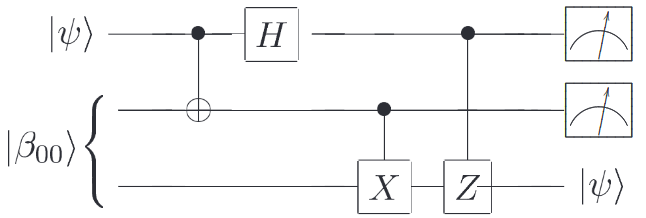
\includegraphics[width=0.6\textwidth]{figures/S2/EJEMPLOCIRCUITO.png}
\caption{\label{fig:CircuitExample} Ejemplo de circuito cuántico. Fuente: \cite{nielsen_chuang_2010}}
\end{figure}

Un circuito cuántico no es otra cosa que un conjunto de \textit{qubits} a los cuales se les aplican compuertas de manera secuencial, ver imagen \ref{fig:CircuitExample}. Los \textit{qubits} son representados como líneas horizontales, dotándoles así de una secuencialidad a la hora de aplicarles compuertas. Al tener varios \textit{qubits}, estos se representan como líneas horizontales paralelas. Usando la notación visual de las compuertas, ver figura \ref{fig:GatesGraphical}, las compuertas son colocadas encima de las líneas, indicando así que esta fue aplicada a ese \textit{qubit}.

Un detalle importante es que si bien los \textit{qubits} son representados de forma paralela, esto no es necesariamente la topología real que tienen, por ejemplo, cuando se simularan los \textit{qubits}, estos tienen conexiones para todos los otros, esto en representación de grafos corresponde a un grafo completo, en el caso de máquinas reales, no todos los \textit{qubits} se pueden conectar con todos (va a estar delimitado por el \textit{hardware}).

\begin{figure}[H]
\centering
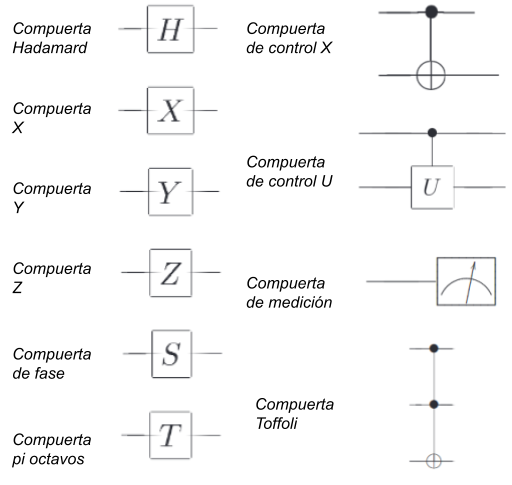
\includegraphics[width=0.7\textwidth]{figures/S2/COMPUERTASVISUAL.png}
\caption{\label{fig:GatesGraphical} Notación gráfica de las compuertas cuánticas. Fuente: \cite{nielsen_chuang_2010}}
\end{figure}

Finalmente, un algoritmo cuántico no es otra cosa que un circuito cuántico cuyas compuertas son elegidas con el objetivo de maximizar las probabilidades de un conjunto de estados que corresponden a la solución del problema. Un tipo famoso de algoritmos en la época NISQ son los algoritmos híbridos, estos son algoritmos con una parte cuántica y una parte clásica, la parte cuántica suele corresponder a la construcción y ejecución de un \textit{ansatz} (término que se explicara más adelante, pero entiéndase como una matriz con parámetros) y la parte clásica es la resolución de un problema de minimización de los parámetros del \textit{ansatz} utilizando algún algoritmo clásico de optimización.

%
%
%
%
%


\newpage
\subsection{Principios básicos y campos de investigación de la materia en estado sólido} 

Esta sección no es una introducción ni a la materia condensada ni a la termodinámica ni a la química cuántica, se asumirá que el lector tiene conocimientos básicos de mecánica cuántica, termodinámica y química. La idea es solo presentar conceptos claves para el desarrollo de la memoria.


\subsubsection{Un poco de química}

Antes de pasar a hablar de como interactúan muchos átomos, es necesario partir hablando de solo uno. La pregunta que surge naturalmente es ¿Qué es un átomo?, un átomo se encuentra compuesto por electrones, protones y neutrones que interactúan entre sí, entonces, nuestros elementos bases para estudiar la materia y su comportamiento van a ser los electrones, protones y neutrones.


Lo primero que hay que revisar es el cómo se construyen los átomos. A la fecha, en la tabla periódica se informan 120 elementos, que difieren en el número atómico, como cada átomo tiene un número diferente de electrones, entonces, la pregunta es ¿cómo se distribuyen estos electrones para formar el átomo?, para ello, debemos introducir el concepto de estructura electrónica de los átomos. 

Como bien se sabe, los electrones en un átomo tienen cuatro números cuánticos ($n$, $l$, $m_l$ y $m_s$), los primeros tres describen la región en donde es más probable encontrar al electrón y el último indica la orientación de su espín. Los electrones son agrupados dentro de capas que están determinadas por el núcleo del átomo, cuanto más grande sea, mayor será el número de capas (por lo tanto, mayor número de electrones). Cada capa tiene un número de subcapas, las cuales contienen un conjunto finito de orbitales. Un orbital no es otra cosa que una región dentro de un átomo en donde un electrón puede ser encontrado, cada orbital puede contener un número finito de electrones.

Cada orbital tiene un número de sitios que pueden ser ocupados por los electrones, el orbital $s$ tiene un sitio, él $d$ tiene tres sitios, él $p$ tiene 5 sitios y él $f$ tiene 14 sitios. Cada sitio puede contener dos electrones, los cuales, por el principio de exclusión de Pauli, deben tener un número cuántico $m_s$ distinto.

Con lo anterior expuesto, podemos pasar a hablar de la estructura electrónica, la cual, no es otra cosa que un arreglo de los electrones sobre las distintas capas. Para ello presentaremos las reglas de Hund y el principio de Aufbau.

El principio de Aufbau fue formulado por Niels Bohr y Wolfgang Pauli en el año 1920, en él se indica que para que los electrones ocupen orbitales de mayor energía deben ocupar por completo los orbitales de menor energía. Por ejemplo, para que los electrones ocupen un orbital $p$, deben ocupar todos los orbitales $s$. Por otro lado, las reglas de Hund son un conjunto de postulados derivados de forma empírica, estos fueron presentados alrededor del 1927 por Friedrich Hund. Las reglas son las siguientes
\begin{enumerate}
    \item El estado de mínima energía es aquel con la mayor multiplicidad del espín.
    \item Para términos con la misma multiplicidad del espín, aquel con el orbital de mayor momento angular, será él con menor energía.
\end{enumerate}

\subsubsection{Modelos sobre el comportamiento de los átomos}
Lo siguiente que tenemos que revisar es el cómo se modelan estas interacciones entre las partículas que componen a los átomos. La expresión general\cite{szabo1996modern} tiene en cuenta todas las posibles interacciones, las cuales se reflejan en las distintas sumatorias de la expresión.

\begin{equation*}
    \mathcal{H} = -\sum_{i=!}^{N}\frac{1}{2}\nabla_i^2 - \sum_{A = 1}^{M} \frac{1}{2M_A}\nabla_A^{2} -\sum_{i=1}^{N}\sum_{A = 1}^{M} \frac{Z_A}{r_{iA}} + \sum_{i=1}^{N}\sum_{j>i}^{N} \frac{1}{r_{ij}}  + \sum_{A=1}^{M}\sum_{B>A}^{M} \frac{Z_AZ_B}{R_{AB}}
\end{equation*}

El problema de esta expresión es el número de grados de libertad y de interacciones que considera, en estructuras complejas es computacionalmente inviable trabajar directamente con esta expresión. Frente a este problema, se han propuesto diferentes aproximaciones que se concentran en modelar características concretas de la materia, lo cual permite reducir la cantidad de grados de libertad (además de considerar ciertos supuestos sobre las interacciones). Una de las aproximaciones más famosa es la de Born-Oppenheimer\cite{BornOppenheimer} donde la idea es que como las partículas del núcleo son más pesadas que los electrones, entonces su velocidad es comparablemente menor que la de los electrones, entonces los términos de la energía cinética y la energía de repulsión (este término se vuelve constante) del núcleo pueden ser despreciados (este se conoce como hamiltoniano electrónico). De esta forma, la expresión anterior se reduce a la siguiente
\begin{equation*}
    \mathcal{H}_{elec} = -\sum_{i=!}^{N}\frac{1}{2}\nabla_i^2  -\sum_{i=1}^{N}\sum_{A = 1}^{M} \frac{Z_A}{r_{iA}} + \sum_{i=1}^{N}\sum_{j>i}^{N} \frac{1}{r_{ij}}
\end{equation*}

De este tipo de aproximaciones es que surgieron diferentes tipos de hamiltonianos que buscan modelar interacciones concretas. acá solo expondremos un par de hamiltonianos. El primer corresponde al hamiltoniano electrónico (también conocido como hamiltoniano de Coulomb) antes mostrado, pero en su forma de segunda cuantización\cite{szabo1996modern}:
\begin{equation}
    \mathcal{H} = \sum_{pq} h_{pq} a^{\dag}_{p} a_{q}  + \frac{1}{2} \sum_{pqrs}h_{pqrs} a^{\dag}_{p}a^{\dag}_{q} a_{r}a_{s}
    \label{eq:SCmolecular}
\end{equation}
Las constantes que acompañan a cada término se definen como las siguientes integrales $h_{pq} = \int \phi^{*}_p(r)(-\frac{1}{2} \nabla^{2} - \sum_I \frac{Z_I}{R_I-r})\phi_q(r) dr$ y $h_{pqrs} = \int \frac{\phi^{*}_p(r_1) \phi^{*}_q(r_2) \phi_r(r_2) \phi_s(r_1) }{|r_1 -r_2|} dr_1 dr_2$.


El siguiente modelo es el Modelo de Heisenberg\cite{Heisenberg1928}, este fue propuesto por Werner Heisenberg para estudiar los cambios de fase y puntos críticos de materiales magnéticos. La expresión matemática del modelo es la siguiente:
\begin{equation}
    \mathcal{H} = \sum_{\<i,j\>} -J \cdot S_i\cdot S_j = \sum_{\<i,j\>} -J^x_{ij}(\sigma^x_i\sigma^x_j) -J^y_{ij}(\sigma^y_i\sigma^y_j) -J^z_{ij}(\sigma^z_i\sigma^z_j)
    \label{eq:Heisenberg}
\end{equation}
En este caso, los espines son modelados usando las matrices de Pauli correspondientes al espín. Este modelo, a pesar de su simpleza, describe bien el comportamiento de sistemas sintetizados y que se encuentran en la naturaleza, además es utilizado para el estudio de transiciones de fase cuántica, superconductividad, entre otras\cite{IntroHeisenberg}. 

Finalmente, el último modelo es el modelo de Hubbard\cite{HubbardModel}. John Hubbard propuso este modelo para modelar el efecto de las correlaciones en las bandas de energía. A continuación, se muestra la ecuación del modelo de Hubbard utilizando operadores de segunda cuantización.
\begin{equation}
    \mathcal{H} = -t \sum_{\expval{i,j}, \sigma}( a^{\dag}_{i, \sigma} a_{j, \sigma} + h.c) + U\sum_{j}n_{j\uparrow}n_{j\downarrow}
    \label{eq:FHHamiltonian}
\end{equation}
El término $t$ corresponde a la energía cinética de los electrones, mientras que el término $U$ corresponde a la interacción efectiva. Una de las motivaciones por estudiar este modelo, es que a pesar de su simpleza, captura bien los fenómenos cuánticos de sistemas con parámetros de características más generales\cite{HubbardModelBook}. Un detalle importante es que con $U = 0$ se obtiene el modelo de \textit{tight-binding}, así que, por comodidad, ambos modelos serán considerados como el mismo.


Todos estos modelos están expresados en su forma más elemental, se le pueden agregar más interacciones para hacer de estos algo más completo y realista, pero, todo esto dependerá de lo que se quiere estudiar.


\subsubsection{Mediciones}

El siguiente tema por tratar es el cómo extraer información útil de los sistemas, existen muchas técnicas experimentales que permiten cuantificar características del sistema, como la espectroscopia, la fluorescencia, entre otros. El problema con esto es que esas técnicas pertenecen al dominio de la física experimental, para efectos de esta memoria, nos concentraremos en las descripciones matemáticas de ciertas cantidades, conocidas en la literatura como observables, las cuales pueden ser calculadas numéricamente teniendo el hamiltoniano. En esta sección presentaremos algunas de las más relevantes y utilizadas en la literatura, para ello tengamos en mente que tenemos un hamiltoniano arbitrario $\mathcal{H}$.

El valor esperado de un operador $O$ con consideración de la temperatura se define como:
\begin{equation*}
    \expval{O} = Tr[\rho O] = \frac{1}{Z}\sum_i \exp{\frac{-E_i}{k_bT}}\bra{\psi_i}O\ket{\psi_i}
\end{equation*}
Donde $\rho = \frac{1}{Z}\sum_i \exp{\frac{-E_i}{k_bT}}\ket{\psi_i}\bra{\psi_i}$. Independiente de la expresión, se requiere tener de forma obligatoria los $E_i$ y $\ket{\psi_i}$ que corresponden a los valores y vectores propios del hamiltoniano, por otro lado, el término $Z$ corresponde a función de partición que se define como $Z = \sum_i \exp{\frac{-E_i}{k_bT}}$ (la cual permite normalizar las exponenciales) y por último, $k_b$ que corresponde a la constante de Boltzmann.

Un caso particular es cuando $T=0$, y es un punto donde solo los estados de mínima energía pueden sobrevivir (los otros estados tienen probabilidades nulas). De igual forma, uno, puede calcular valores esperados usando un solo estado, por ejemplo, el de mínima energía bajo el supuesto de trabajar a temperatura 0 o un estado que evoluciona respecto al tiempo. Matemáticamente, esto se define como:

\begin{equation*}
    \expval{O} = \bra{\psi} O \ket{\psi}
\end{equation*}

Existe una gran cantidad de observables\cite{EfectoMagnetocalorico}, pero para esta memoria nos enfocaremos en dos observables, la magnetización y el calor especifico. La magnetización suele estudiarse en sistemas de espines y se busca caracterizar la orientación de estos, en ese caso se considera una magnetización parcial, ya que nos concentramos en un subconjunto.
\begin{equation*}
    \expval{M} = \sum_i \expval{m_i} = \sum_i \frac{1}{Z}(\sum_j \exp{\frac{-E_j}{Tk_b}} \bra{E_j}m_i\ket{E_j})
\end{equation*}
Los términos $m_i$ corresponden a la magnetización en cada sitio, de forma individual. Por otro lado, el calor específico se define como la cantidad de energía necesaria para elevar la temperatura de un material en una unidad, matemáticamente se define de la siguiente forma:
\begin{equation*}
    c_b = \frac{\expval{\mathcal{H}^2}- \expval{\mathcal{H}}^2}{T^2k_b}
\end{equation*}

Un detalle que es necesario aclarar es hay que tener cuidado a la hora de calcular un observable a un hamiltoniano, ya que, se debe tener en cuenta que el observable tiene sentido en este.

\subsection{Codificación y trabajo en el espacio de espines}

\subsubsection{Codificación de Jordan Wigner}
Esta es una de las codificaciones más intuitivas que permiten conectar operadores de segunda cuantización con operadores de espines. La idea es utilizar que las matrices de Pauli conforman una base del espacio de matrices de $2x2$, por lo tanto, es posible generar una descomposición en esta base de los diferentes operadores. Dicho esto, a continuación se mostrarán equivalencias de los operadores de creación y aniquilación respectivamente (las operaciones omitidas son los productos Kronecker) \cite{Lana}:
\begin{equation*}
    a_j^{\dag} = \sigma_0^Z \cdots \sigma^Z_{j-1} \frac{1}{2}(\sigma^X_j -i\sigma^Y_j) \sigma^I_{j+1} \cdots \sigma^I_{n} 
\end{equation*}
\begin{equation*}
    a_j = \sigma^Z_0 \cdots \sigma^Z_{j-1}  \frac{1}{2}(\sigma^X_j +i\sigma^Y_j) \sigma^I_{j+1} \cdots \sigma^I_{n}
\end{equation*}
Con estas dos equivalencias, es posible derivar las representaciones en el espacio de espines de los otros operadores (como el número de partículas entre otros). Una de las características más relevantes de esta nueva representación, es que todos los operadores de segunda cuantización pueden ser expresados como un producto tensorial de sistemas aislados. 

Dentro de la literatura existen otras codificaciones más eficientes, respecto al número de \textit{qubits} necesarios, como la de Bravyi-Kitaev y de paridad \cite{JW-BK-COD}.

\subsubsection{Ejemplo de representación de hamiltonianos}

Para ejemplificar el cómo utilizar esta transformación, tomaremos el hamiltoniano en segunda cuantización para el dímero de hidrógeno (distancia de $0.775$ (ángstrom) y basis set ''sto-3g''), el cual se resume en la siguiente expresión:

\begin{multline*}
     \mathcal{H} = -1.25633( a_0^{\dag} a_0 ) + -0.47189( a_1^{\dag} a_1 ) + -1.25633( a_2^{\dag} a_2 ) + -0.47189( a_3^{\dag} a_3 ) \\
+ 0.33785( a_0^{\dag}a_0^{\dag} a_0 a_0 ) + 0.09046( a_0^{\dag} a_0^{\dag} a_1 a_1 ) + 0.09046( a_0^{\dag} a_1^{\dag} a_0 a_1 ) + 0.33229( a_0^{\dag} a_1^{\dag} a_1 a_0 ) \\
+ 0.33785( a_0^{\dag} a_2^{\dag} a_2 a_0 ) + 0.09046( a_0^{\dag} a_2^{\dag} a_3 a_1 ) + 0.09046( a_0^{\dag} a_3^{\dag} a_2 a_1 ) + 0.33229( a_0^{\dag} a_3^{\dag} a_3 a_0 ) \\
+ 0.33229( a_1^{\dag} a_0^{\dag} a_0 a_1 ) + 0.09046( a_1^{\dag} a_0^{\dag} a_1 a_0 ) + 0.09046( a_1^{\dag} a_1^{\dag} a_0 a_0 ) + 0.34928( a_1^{\dag} a_1^{\dag} a_1 a_1 ) \\
+ 0.33229( a_1^{\dag} a_2^{\dag} a_2 a_1 ) + 0.09046( a_1^{\dag} a_2^{\dag} a_3 a_0 ) + 0.09046( a_1^{\dag} a_3^{\dag} a_2 a_0 ) + 0.34928( a_1^{\dag} a_3^{\dag} a_3 a_1 ) \\
+ 0.33785( a_2^{\dag} a_0^{\dag} a_0 a_2 ) + 0.09046( a_2^{\dag} a_0^{\dag} a_1 a_3 ) + 0.09046( a_2^{\dag} a_1^{\dag} a_0 a_3 ) + 0.33229( a_2^{\dag} a_1^{\dag} a_1 a_2 ) \\
+ 0.33785( a_2^{\dag} a_2^{\dag} a_2 a_2 ) + 0.09046( a_2^{\dag} a_2^{\dag} a_3 a_3 ) + 0.09046( a_2^{\dag} a_3^{\dag} a_2 a_3 ) + 0.33229( a_2^{\dag} a_3^{\dag} a_3 a_2 ) \\
+ 0.33229( a_3^{\dag} a_0^{\dag} a_0 a_3 ) + 0.09046( a_3^{\dag} a_0^{\dag} a_1 a_2 ) + 0.09046( a_3^{\dag} a_1^{\dag} a_0 a_2 ) + 0.34928( a_3^{\dag} a_1^{\dag} a_1 a_3 ) \\
+ 0.33229( a_3^{\dag} a_2^{\dag} a_2 a_3 ) + 0.09046( a_3^{\dag} a_2^{\dag} a_3 a_2 ) + 0.09046( a_3^{\dag} a_3^{\dag} a_2 a_2 ) + 0.34928( a_3^{\dag} a_3^{\dag} a_3 a_3 ) 
\end{multline*}

Tomando el término $a_0^{\dag} a_0$. Si aplicamos la transformación de Jordan-Wigner considerando $n=4$, tenemos el siguiente producto:

\begin{equation*}
    a_0^{\dag} a_0 = (\frac{1}{2}(\sigma^X_0 -i\sigma^Y_0)\otimes\sigma^I_1\otimes\sigma^I_2\otimes\sigma^I_3) (\frac{1}{2}(\sigma^X_0 +i\sigma^Y_0)\otimes\sigma^I_1\otimes\sigma^I_2\otimes\sigma^I_3)
\end{equation*}

Como solo el primer sitio tiene operadores distintos a la identidad, podemos desarrollar el producto, llegando a $(\sigma^X_0 -i\sigma^Y_0)(\sigma^X_0 +i\sigma^Y_0) = 2\sigma_0^I + i\sigma_0^X\sigma_0^Y - i\sigma_0^Y\sigma_0^X$. Entonces, el término original es representado en el espacio de espines como (se omitirán los productos tensoriales):

\begin{equation*}
    a_0^{\dag} a_0 = \frac{1}{2}\sigma^I_0\sigma^I_1\sigma^I_2\sigma^I_3 + \frac{i}{4}(\sigma^X_0\sigma^Y_0)\sigma^I_1\sigma^I_2\sigma^I_3 - \frac{i}{4}(\sigma^Y_0\sigma^X_0)\sigma^I_1\sigma^I_2\sigma^I_3
\end{equation*}


Siguiendo este procedimiento con el resto de los términos, podemos reescribir el hamiltoniano de segunda cuantización en el espacio de espines, el cual es mostrado a continuación:

\begin{multline*}
\mathcal{H} = -0.81054\sigma_0^I\sigma_1^I\sigma_2^I\sigma_3^I + 0.17218\sigma_0^I\sigma_1^I\sigma_2^I\sigma_3^Z - 0.22575\sigma_0^I\sigma_1^I\sigma_2^Z\sigma_3^I \\
+ 0.17218\sigma_0^I\sigma_1^Z\sigma_2^I\sigma_3^I - 0.22575\sigma_0^Z\sigma_1^I\sigma_2^I\sigma_3^I + 0.12091\sigma_0^I\sigma_1^I\sigma_2^Z\sigma_3^Z \\
+ 0.16892\sigma_0^I\sigma_1^Z\sigma_2^I\sigma_3^Z + 0.04523\sigma_0^Y\sigma_1^Y\sigma_2^Y\sigma_3^Y + 0.04523\sigma_0^X\sigma_1^X\sigma_2^Y\sigma_3^Y \\
+ 0.04523\sigma_0^Y\sigma_1^Y\sigma_2^X\sigma_3^X + 0.04523\sigma_0^X\sigma_1^X\sigma_2^X\sigma_3^X + 0.16614\sigma_0^Z\sigma_1^I\sigma_2^I\sigma_3^Z \\
+ 0.16614\sigma_0^I\sigma_1^Z\sigma_2^Z\sigma_3^I + 0.17464\sigma_0^Z\sigma_1^I\sigma_2^Z\sigma_3^I + 0.12091\sigma_0^Z\sigma_1^Z\sigma_2^I\sigma_3^I
\end{multline*}

Ambos hamiltonianos son equivalentes y reflejan la misma física del sistema. Lo importante de esta transformación es que el segundo hamiltoniano es más fácil de construir y trabajar en computador, ya que, que los operadores de espines tienen descripciones matriciales directas a diferencia de los operadores de segunda cuantización.


%
%
%
%
%
\subsection{Como utilizar los ordenadores cuánticos para hacer física}
En esta sección, se presentarán los componentes básicos para poder extraer física de los cálculos realizados dentro de los circuitos cuánticos.

\subsubsection{\textit{Ansatz}}
Uno puede definirse un estado arbitrario con el cual partir el circuito, pero para poder conectarlo con el problema, es necesario que exista una serie de compuertas que permitan ir variando este estado inicial y que se ajuste a lo que buscamos. Esta descripción se conoce normalmente como \textit{ansatz}, estos suelen estar parametrizados por un vector $\theta$, donde las componentes son valores que permiten ir ajustando la rotación derivada de las compuertas del \textit{ansatz} ($\ket{\psi(\theta)} = U(\theta)\ket{\psi_0}$). De esta forma, es posible ir ajustando los parámetros para que nuestro vector inicial se ajuste al problema que intentamos solucionar. 

Los \textit{ansatz} son altamente utilizados en los algoritmos variacionales cuánticos, ya que, el \textit{ansatz} puede ser simulado de forma eficiente en un ordenador cuántico. Una de las limitaciones de los \textit{anzats}, es que, como son responsables de generar el espacio de posibles estados, una elección incorrecta del mismo puede derivar en soluciones sin sentido. A continuación, se mostrarán los \textit{ansatz} más utilizados en la literatura.

El \textit{hardware efficient ansatz}\cite{EfficientAnsatz} corresponde a uno de los tipos de \textit{ansatz} más generales y fue diseñado para ser implementado en dispositivos NISQ. La idea es descomponer un operador unitario local genérico como el producto de las compuertas de rotación $R_x, R_y$ y $R_z$, uno de los problemas de esto es el crecimiento del número de parámetros necesario, ya que, por cada compuerta se requieren $3$ parámetros, lo cual, para $n$ \textit{qubits} y una profundidad $D$ se requieren $3nD$ \textit{qubits}.
\begin{equation*}
    U(\theta) = \prod_{d=1}^{D} U_{ent} \prod_{i=1}^{n} R_z(\theta_1^{i,d})R_x(\theta_2^{i,d})R_y(\theta_3^{i,d})
\end{equation*}
Este \textit{ansatz} tiene un buen rendimiento para un bajo número de \textit{qubits} (2-6), pero presenta un problema de desvanecimiento del gradiente a medida que se aumenta el número de \textit{qubits}, en ratio de decrecimiento es de tipo exponencial\cite{DesvanecimientoGradiente}. 

El \textit{unitary coupled cluster} (UCC)\cite{doi:10.1021/acs.jctc.8b01004}\cite{Fedorov2022} es utilizando en el contexto de química cuántica y materia condensada. A diferencia del \textit{ansatz} anterior, en este sí incluye contexto del problema, considerando los orbitales de las moléculas. El \textit{coupled cluster} tradicional se define de la siguiente manera
\begin{equation*}
    \hat{T} = \hat{T_1} + \hat{T_2} = \sum_{i,a} t_i^a \hat{a_a}^{\dag} \hat{a_i} + \frac{1}{4}\sum_{i,j,a,b} t_{ij}^{ab} \hat{a_a}^{\dag} \hat{a_b}^{\dag} \hat{a_j}\hat{a_i}
\end{equation*}
Este puede tener más términos, pero para efectos practicas con dos son suficientes. Lamentablemente, al aplicarle la exponencial a $\hat{T}$, lo que se obtiene no es un operador unitario, por lo tanto, no puede ser representado como un circuito. Por lo tanto, para definir el \textit{ansatz} se define de la siguiente forma:
\begin{equation*}
    U = exp(\hat{T} - \hat{T}^{\dag})
\end{equation*}
Este se conoce como \textit{Unitary Coupled Cluster Single Doubles} (UCCSD), luego tenemos otra variante llamada \textit{k-Unitary pair Coupled Cluster Generalized Singles and Doubles Product Wavefunctions} (k-UpCCGSD), la cual se define de mediante la siguiente productoria:
\begin{equation*}
    U = \prod_{\alpha=1}^{k} exp(\hat{T^{\alpha}} - \hat{T^{\alpha}}^{\dag}) 
\end{equation*}
La diferencia respecto al anterior sobre el término $\hat{T_2}$, el cual se define de la siguiente forma:
\begin{equation*}
    \hat{T_2} = \sum_{i,\alpha} t_{i_{\alpha} i_{\beta}}^{a_{\alpha} a_{\beta}} \hat{a}^{\dag}_{a_{\alpha}} \hat{a}^{\dag}_{a_{\beta}} \hat{a}_{i_{\beta}} \hat{a}_{i_{\alpha}}
\end{equation*}

Ambos, como su nombre indican, solo consideran interacciones individuales y entre pares, es posible extender estos \textit{ansatz} para que consideren más interacciones, lo cual no es otra cosa que agregar más términos $\hat{T_i}$.

El \textit{variational hamiltonian ansatz} \cite{PhysRevA.92.042303} se presenta como una alternativa al UCC para situaciones en las que se conoce que la precisión del UCC falla (grandes moléculas con un acople fuerte), la idea base es, reescribir y entender el hamiltoniano como una sumatoria de sub hamiltonianos.
\begin{equation*}
    H = \sum_i J_i H_i
\end{equation*}
De esta forma, es posible escribir el \textit{ansatz} como una productoria de la exponencial de cada uno de estos sub hamiltonianos, el detalle importante, es que esta separación en una productoria es posible usando la Troterizacion de la exponencial.
\begin{equation*}
    exp(-itH) = exp( -it\sum_j J_j H_j ) = ( \prod_j exp(-i\frac{\theta}{r} H_j) )^r
\end{equation*}
A diferencia de los \textit{ansatz} anteriores, acá se tiene en consideración toda la información del sistema y por ello es más difícil de construir, ya que, si no se construye adecuadamente puede conllevar un circuito de mucha profundidad.


En los últimos años, se ha propuesto un nuevo tipo de \textit{ansatz} diferente a los mencionados anteriormente, los anteriores caen en la categoría de \textit{ansatz} de estructura fija, este nuevo tipo se conoce como \textit{ansatz} de estructura adaptativa \cite{ADAPTVQE}.


\subsubsection{Valor esperado en la base computacional}
Como todos los operadores de los hamiltonianos antes definidos pueden ser reescritos en términos de un producto tensorial de matrices de Pauli, nos interesa conocer el cómo calcular el valor esperado de ese producto. Una buena noticia es los \textit{qubits} se miden en él $Z$, por lo tanto, a las expresiones con términos $X$ y $Y$ tienen que ser reescritas en el eje $Z$ (en el caso de $X$ aplicando una compuerta $H$ en los \textit{qubit} que se miden, y en el caso de $Y$ se aplica una compuerta $S$ seguida de una $H$).

Resumiendo, al final lo único que nos importa es como calcular el valor esperado para el operador compuesto por matrices $Z$, ya que, los circuitos se miden en este eje. Antes de partir, definimos $\ket{\psi}$  como un estado arbitrario de $n$ \textit{qubits}.

Para el caso de un \textit{qubit} ($n=1$), podemos descomponer el operador $Z = \ket{0}\bra{0} - \ket{1}\bra{1}$, ahora si le calculamos el valor esperado:
\begin{equation*}
    \expval{Z} = \bra{\psi} (\ket{0}\bra{0} - \ket{1}\bra{1}) \ket{\psi} = |\bra{0}\ket{\psi}|^2 -  |\bra{1}\ket{\psi}|^2
\end{equation*}
Donde los $|\bra{i}\ket{\psi}|^2$ no son más que las probabilidades asociadas de colapsar en ese estado basal.

Para dos \textit{qubits} ($n=2$) la idea es exactamente la misma, descomponemos el operador $Z \otimes Z =\ket{00}\bra{00} - \ket{01}\bra{01} - \ket{10}\bra{10} + \ket{11}\bra{11}$ y si le calculamos el valor esperado vamos a obtener lo siguiente:
\begin{equation*}
    \expval{Z \otimes Z}  = |\bra{00}\ket{\psi}|^2 - |\bra{01}\ket{\psi}|^2 -  |\bra{10}\ket{\psi}|^2 + |\bra{11}\ket{\psi}|^2
\end{equation*}

Ahora la pregunta es, como se calculan para $n$ operadores $Z$. Por temas de notación, denotaremos a este operador como $Z^{\otimes n}$, este se puede descomponer como:
\begin{equation*}
    Z^{\otimes n} = \sum_{ i \in \{ 0,1\}^{n}} (-1)^{p(i)}\ket{i}\bra{i}
\end{equation*}
Donde la función $p(i)$ determina la paridad, que en este caso, es la cantidad de 1 dentro del estado, por ejemplo, para el estado $x = \ket{110}$, la función $p(x)=0$ porque hay un número par de 1. Entonces, si le calculamos el valor esperado, obtenemos la siguiente fórmula:
\begin{equation*}
    \expval{Z^{\otimes n}} = \sum_{ i \in \{ 0,1\}^{n}} (-1)^{p(i)}|\bra{i}\ket{\psi}|^2
\end{equation*}

Hay un caso particular que es cuando hay matrices $I$ dentro del producto tensorial. De forma práctica, estas se pueden ignorar al momento de la medición y concentrarse en aquellos \textit{qubits} donde según el operador hay una acción, por ejemplo, para el operador $Z \otimes I \otimes Z$ bastaría medir el primer y el último \textit{qubit}, y aplicar la fórmula para dos \textit{qubits}. Esto es particularmente útil cuando se trabaja con hamiltonianos de espines, ya que estos solo suelen tener dos términos dentro de cada sub hamiltoniano que son distintos a $I$.



\subsection{Métodos híbridos}
Luego de hacer un repaso por algunos conceptos importantes, podemos volver al tema de los algoritmos híbridos. Debido a que nos encontramos en la era NISQ (a la fecha de escrita la memoria), las máquinas actuales no son capaces de manejar correctamente el error a un gran número de \textit{qubits} y hacen que los métodos híbridos sean la mejor opción. 


\subsubsection{\textit{Variational quantum eigensolver}}
El Corresponde \textit{variational quantum eigensolver} (VQE) \cite{VQE} a uno de los algoritmos híbridos más famosos dentro de la era NISQ, su objetivo es el poder calcular el valor de mínima energía de un hamiltoniano, utilizando un \textit{ansatz} para construir los posibles estados y una función de coste para poder encontrar el valor óptimo de los parámetros del \textit{ansatz}, estos valores óptimos son los que entregan la mínima energía, ya que, la función de coste está acotada $E_0 \leq \mathcal{L}(\theta)$.

Este \textit{ansatz} es un circuito cuántico parametrizado y la minimización de la función de coste es llevada a cabo por un algoritmo de minimización clásico. La función de coste que se minimiza es la siguiente:
\begin{equation*}
    \mathcal{L}(\theta) = \bra{\psi_0}U^{\dag}(\theta)\mathcal{H}U(\theta)\ket{\psi_0}
\end{equation*}



A pesar de su simpleza, este método tiene diversas aplicaciones, una de las principales a la fecha es el de caracterizar el estado actual y a su vez ayudar a construir \textit{benchmark} \cite{McCaskey2019QCbench}. además de estas, nos interesa la optimización de las distancias moleculares en hamiltonianos moleculares\cite{OptimizationStruture}, esta optimización no es otra cosa que encontrar las distancias entre moléculas que entregan un equilibrio. Para lograr esto, se extiende la función de coste anterior (la función del VQE), agregando un nuevo conjunto de parámetros que representan las posiciones de las moléculas en un espacio 3D.

\begin{equation*}
    \mathcal{L}(\theta, x) = \bra{\psi_0}U^{\dag}(\theta)\mathcal{H}(x)U(\theta)\ket{\psi_0}
\end{equation*}

Al final, lo que se busca es parametrizar el hamiltoniano y calcular las constantes en función de la distancia de los átomos (en este caso se habla de las constantes del hamiltoniano de espines formadas por la transformación de Jordan Wigner o de Bravyi-Kitaev aplicada al hamiltoniano molecular), ya que los orbitales no varían, solo el valor de las constantes.

\begin{equation*}
    \mathcal{H}(x) = \sum_i J_i(x)h_i
\end{equation*}

Con el hamiltoniano parametrizado, se busca encontrar las posiciones en el espacio que $\nabla_x E=0$, indicando así que nos encontramos en un mínimo que no es otra cosa que la estructura en un estado de equilibrio. Usando la función de coste, podemos encontrar la estructura que ofrece el valor de mínima energía junto a lo que nos entrega el VQE.



\subsubsection{\textit{Variational quantum deflation}}
El \textit{variational quantum deflation} (VQD) \cite{Higgott2019variationalquantum} surge como una respuesta a la pregunta de cómo obtener los niveles excitados de un hamiltoniano, es decir, se extiende el VQE para que sea capaz de calcular los niveles excitados.

La idea es utilizar el solapamiento para modificar el hamiltoniano, consideremos $\ket{E_0}$ como el estado de mínima energía de un hamiltoniano $\mathcal{H}$, por lo tanto, lo siguiente es reescribir el hamiltoniano de la siguiente forma:
\begin{equation*}
    \mathcal{H}^{\prime} = \mathcal{H} + \beta\ket{E_0}\bra{E_0}
\end{equation*}
Con $\beta \gg 0$. Lo interesante de este nuevo hamiltoniano es su nuevo estado de mínima energía, es $\ket{E_1}$ del hamiltoniano original. Esta idea puede extenderse para calcular todos los estados del sistema, simplemente habrá que agregar más términos de solapamiento.


Esta idea puede resumirse en la siguiente función de coste.
\begin{equation*}
    \mathcal{L}(\theta_k) = \bra{\psi_0}U^{\dag}(\theta_k)\mathcal{H}U(\theta_k)\ket{\psi_0} + \sum_{i=0}^{k-1}\beta_i |\bra{\psi_0}U^{\dag}(\theta_i)U(\theta_k)\ket{\psi_0} |^{2}
\end{equation*}

El primer término no es otra cosa que la energía respecto al hamiltoniano, pero lo interesante es el término de la sumatoria, este refleja el solapamiento de estados, la idea es que este término funcione como una penalización para que el algoritmo de minimización busque estados que sean ortogonales al estado anterior calculado (considerando que el primer estado es el de mínima energía, la idea es que los estados siguientes sean ortogonales entre sí, es decir que sean vectores propios, solo así, el término de penalización es 0).



\subsubsection{\textit{Variational quantum thermalizer}}
El \textit{variational quantum thermalizer} (VQT) \cite{VQT} responde a la necesidad como introducir la temperatura dentro de los cálculos. Por lo tanto, el objetivo es completamente distinto a los otros métodos, acá no se busca capturar los estados del hamiltoniano, acá se busca capturar el operador de densidad termodinámico (aquel que genera la distribución de probabilidades basándonos en la temperatura).

La función de coste asociada a este método es la siguiente:

\begin{equation*}
    \mathcal{L}(\theta, \phi) = \frac{1}{T} Tr[\mathcal{H}U^{\dag}_\phi \rho_\theta U_\phi] - S(\rho_\theta)
\end{equation*}

El primer término no es otra cosa que el valor esperado expresado como la traza del producto entre hamiltoniano y el operador de densidad, el otro término consiste en la entropía de Von Neumann sobre la distribución dada por el operador de densidad. Al igual que en el VQE, el objetivo es minimizar esta función, ya que, se tiene la siguiente desigualdad $U^{\dag}_\phi \rho_\theta U_\phi \geq \rho_{termal}$.


\newpage
\secnumbersection{PROPUESTA DE SOLUCIÓN}
En este capítulo se entrega toda la información relacionada con la implementación y desarrollo de la solución. Este capítulo se divide en dos subcapítulos; en el primero se presenta el conjunto de tecnologías y una visión más detallada de la propuesta de solución. El subcapítulo siguiente se centra en aclarar y desarrollar ciertos detalles relevantes de la implementación.


\subsection{Descripción general de la solución}

\subsubsection{Conjunto de tecnologías}
El proyecto se desarrolla usando Python como lenguaje de programación y con el apoyo de librerías especializadas en computación científica y ciencia de datos como NumPy, SciPy, Pandas y Matplotlib. Para trabajar y manipular circuitos cuánticos vamos a utilizar la librería Pennylane\cite{pennylane}.  

La librería Pennylane forma parte del ecosistema de librerías especializadas en el control y la simulación de circuitos cuánticos, esta se diferencia de otras librerías, como Qiskit (desarrollada por IBM) y Cirq (desarrollada por Google), debido a su enfoque en la programación diferencial. Este enfoque permite desarrollar nuevos métodos que permitan ajustar sus parámetros, mejorando así su desempeño y generalidad (editando sus parámetros se pueden ajustar para mejorar su rendimiento en diferentes contextos).

En las siguientes secciones, cuando se hagan referencia a las funciones implementadas dentro de la librería, se utilizará la abreviación de \textit{qml}.

\subsubsection{Visión general del trabajo realizado}
Uno de los problemas de la librería es que implementa muchas funcionalidades y temas de interés, pero estas solo se presentan en modelos de juguete. La labor de software consiste en optimizar y utilizar estos conceptos y funcionalidades para crear modelos y estructuras más complejas.

Para lograr esto, se utiliza una programación con base en clases, estas se pueden agrupar en tres grandes tipos, hamiltoniano, \textit{ansatz} y optimizador (cada una construye objetos diferentes). La razón detrás de esta selección radica en buscar una independencia entre los componentes, en el flujo de los algoritmos variacionales cuánticos, de tal forma que los cambios en el tipo de hamiltoniano, \textit{ansatz}, etc. no genere una mayor repercusión dentro del código, más allá de los parámetros para construir de nuevo la clase. Para entender esto pensemos en que tenemos la clase del \textit{ansatz} UCCSD con la del optimizador genérico, la idea es que si queremos pasar de una estructura molecular al modelo de Fermi-Hubbard, solo tengamos que rehacer la clase del hamiltoniano mientras que la del \textit{ansatz} y optimizador quedan intactas.


El objetivo de la clase de los hamiltonianos es poder construirlo utilizando rutinas de la librería, además de, optimizar el cómo se agrupan los términos para una medición y ejecución de la función de coste más eficiente. La segunda clase se enfoca en crear el circuito y las características con las cuales se ejecutará (si tendrá un entorno con o sin ruido). Finalmente, la clase del optimizador, el cual es un objeto que almacena los hiperparámetros de los optimizadores disponibles en la librería.

A partir de lo anterior, es preciso tener en cuenta que este proyecto no busca ser otra librería que implemente piezas básicas para trabajar con circuitos cuánticos (como Qiskit, Cirq, Pennylane entre otros). Este proyecto pretende implementar flujos de cálculo complejos que permitan utilizar los métodos variacionales cuánticos para estudiar estructuras complejas.


\subsection{Detalles de la implementación}

\subsubsection{Hamiltoniano considerados}
El siguiente asunto es indicar con que hamiltonianos vamos a trabajar. Debido a que, como indicó en el marco teórico, tiene muchas formas de expresarse, considerando más o menos interacciones, por lo tanto, es importante aclarar que parámetros de los hamiltonianos se están considerando.

\begin{figure}[H]
\centering
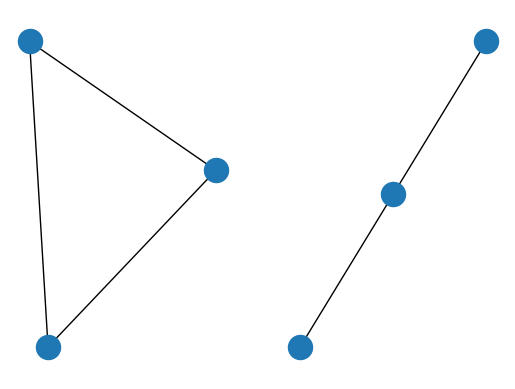
\includegraphics[width=0.5\textwidth]{figures/S3/condiciones.png}
\caption{\label{fig:CBorde} Grilla de estructura de anillo y cadena para 3 sitios respectivamente. Fuente: Elaboración propia}
\end{figure}

\underline{Hamiltoniano molecular}: 
Para el caso del hamiltoniano molecular, se consideran todas aquellas estructuras que pueden ser escritas en términos de elementos atómicos y sus correspondientes posiciones en el espacio, cabe destacar que las posiciones tienen que estar en unidades atómicas. 

Este hamiltoniano está en unidades de energía Hartree y es construido utilizando la función \textit{qml.qchem.molecular\_hamiltonian} (esta función construye el hamiltoniano de la ecuación \ref{eq:SCmolecular}). Para construir el hamiltoniano solo utilizamos el \textit{basis set} ''sto-3g''. El \textit{basis set} es un elemento fundamental en la construcción, ya que, en este, se encuentra la información de las constantes que acompañan los términos del hamiltoniano, ahorrando así tiempos de cálculos (considerando que estas constantes son integrales), el \textit{basis set} elegido corresponde a uno de los más básicos.

\underline{Hamiltoniano Fermi-Hubbard}: 
Para el hamiltoniano de Fermi-Hubbard, ver ecuación \ref{eq:FHHamiltonian}, consideramos las interacciones de \textit{hopping} ($-t$) y las del potencial ($-U$), no hay términos de interacciones externas (véase, un campo magnético y/o eléctrico). El hamiltoniano modela dos tipos de grilla (cadenas y anillos), ver figura \ref{fig:CBorde}.

De manera similar, como el hamiltoniano \textit{tight biding} se deriva del de Fermi-Hubbard considerando $U=0$, este está limitado a las mismas grillas.

La construcción de este hamiltoniano se realiza con las funciones \textit{qml.FermiA} y \textit{qml.FermiC} que implementan los operadores de aniquilación y creación respectivamente (operadores de segunda cuantización), y \textit{qml.jordan\_wigner} que permite después de construir el hamiltoniano en segunda cuantización pasarlo al espacio de espines. Él desafió de esta construcción utilizando estos operadores, poder es construir correctamente las interacciones dadas por las grillas.


\underline{Hamiltoniano espines}: 
Para el hamiltoniano de espines, ver ecuación \ref{eq:Heisenberg}, consideramos un modelo de Heisenberg con una interacción de \textit{exchange} ($J$) homogénea para cada eje, es decir, $J_{ij}^{x} = J_{ij}^{y} = J_{ij}^{z}$ $\forall i,j$ (este hamiltoniano es conocido en la literatura como \textit{quantum Heisenberg model XXX}). No se tiene en consideración campos externos. Este hamiltoniano modela dos tipos de grilla (cadenas y anillos), ver figura \ref{fig:CBorde}.

Este hamiltoniano se construye utilizando la función \textit{qml.pauli.string\_to\_pauli\_word}, que permite construir desde una lista de caracteres un operador, por lo tanto, al igual que en el hamiltoniano anterior, él desafió está en construir las listas que representen la acción de los operadores según la grilla elegida.

En lo que sigue del escrito, cuando se hagan referencia a los modelos, se debe tener en consideración las condiciones expresadas en este capítulo.

\subsubsection{Representación de los hamiltonianos}
Para almacenar los hamiltonianos descritos en el punto anterior, se elige escribirlos en la representación de lista de cadenas de Pauli. Si miramos la fórmula del cálculo del valor esperado (capítulo 2.4.2), no es necesario tener las matrices de forma explícita, como todo se mide respecto al eje Z, solo es necesario saber en qué índices de un término hay que aplicar un cambio de base para medirlo respecto al eje Z. Es por ello, que solo necesitamos un identificador de qué matriz de Pauli se está aplicando en cada sitio, para ello utilizamos el alfabeto $X$, $Y$, $Z$ y $I$, y representamos los términos como un solo \textit{string} compuesto por este alfabeto.

Para entender lo anterior, veamos un ejemplo, tomemos el término $\sigma_0^Z \otimes \sigma_1^Z \otimes \sigma_2^I$, matricialmente, esto es equivalente a una matriz de $8\times 8$, como no estamos utilizando las matrices y solo nos interesa los índices y el identificador, la matriz anterior puede ser representada como la siguiente cadena $''ZZI''$, en donde se refleja que en las primeras posiciones se tiene la acción del operador Z. En caso de tener alguna constante, esta se acopla como una lista, siguiendo el término de ejemplo, quedaría como $[-J, ''ZZI'']$.

Lo anterior es aplicado a cada término del hamiltoniano, permitiendo así una representación que reduce la cantidad de memoria requerida para almacenarla (al no tener que utilizar matrices de forma explícita) y a su vez mantiene toda la información necesaria para el cálculo de valores esperados.

%
%
%
%
%
\subsubsection{\textit{Ansatz} considerados}
Uno de los elementos fundamentales para trabajar con algoritmos variacionales cuánticos son los ansaztz. Para esta memoria consideramos tres \textit{ansatz} de estructura fija, el UCCDS, el k-UpCCGSD y el HE, los cuales serán utilizados en el VQE para estimar el estado y valor de mínima energía.

\underline{UCCDS}:
El primer \textit{ansatz} corresponde al UCCSD, el cual está compuesto por operadores de excitación simples y dobles, estos operadores mantienen constante el número de partículas. Este \textit{ansatz}, por su estructura, no tiene la capacidad de aplicar repeticiones (adjuntar el mismo \textit{ansatz} varias veces dentro del circuito). Este se encuentra implementado en la función \textit{qml.UCCSD}.


\underline{k-UpCCGSD}: 
El segundo \textit{ansatz} se basa en la misma teoría que el anterior (\textit{Unitary Coupled Cluster}), este también se define basándose en operadores de excitación simples y dobles (por lo tanto, también conserva el número de partículas constante), con el detalle de este si admite la posibilidad de generar $k$ repeticiones dentro del circuito. Este se encuentra implementado en la función \textit{qml.kUpCCGSD}


\underline{\textit{Hardware Efficient}}: 
El concepto de \textit{Hardware Efficient} es muy amplio, ya que, hace referencia a compuertas nativas al \textit{hardware}, para esta memoria consideramos una implementación que es afín a hamiltonianos hermíticos, esta se basa en compuertas de rotación $R_Y(\theta)$ y compuertas $CX$, ver figura \ref{fig:RY}. Este \textit{ansatz} es conocido en la literatura como ''\textit{Real amplitudes}'', ya que, al manejar solo esa rotación, estamos dando a entender que los estados solo tendrán amplitudes reales. Ambas compuertas están implementadas en \textit{qml.ry} y \textit{qml.cnot}.

\begin{figure}[H]
\centering
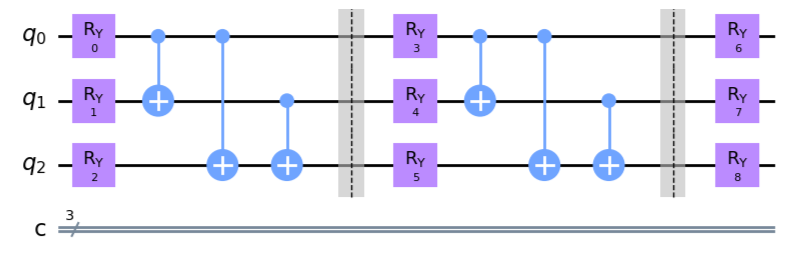
\includegraphics[width=0.8\textwidth]{figures/S2/RYansatz.png}
\caption{\label{fig:RY} Ansatz con compuertas $R_y(\theta)$ y $CX$ para 3 \textit{qubits} hecho en Qiskit. Fuente: Elaboración propia}
\end{figure}

%
%
%
%
%

\subsubsection{Optimizadores considerados}
Al estar trabajando con algoritmos variacionales cuánticos, una parte fundamental son los optimizadores, los cuales son necesarios para ajustar los parámetros del \textit{ansatz}. Para este desarrollo consideramos dos optimizadores, el primero corresponde a un método de gradiente genérico el cual tiene un parámetro de aprendizaje fijo en todo el proceso, el segundo optimizador es ADAM, que es utilizado en trabajos de \textit{machine learning} y \textit{deep learning}, el cual es un optimizador con un parámetro de aprendizaje adaptativo al utilizar los primeros momentos, esto ayuda a evadir problemas de convergencia a medida que se está iterando. 

Ambos optimizadores se encuentran implementados en las funciones \textit{qml.GradientDescentOptimizer} y \textit{qml.AdamOptimizer} respectivamente.


%
%
%
%
%
\subsubsection{Optimización del cálculo de la función de coste}
Uno de los problemas al trabajar con métodos variacionales cuánticos es el tema de la cantidad de ejecuciones del circuito necesarias para evaluar la función de coste. Tomando como ejemplo el hamiltoniano de $H_2O$, este tiene $1086$ términos, en una implementación \textit{naive}, se tendría que ejecutar el circuito $1086$ para poder calcular el valor de la función de coste para ese valor de parámetros. Cuando las estructuras tienen muchos \textit{qubits} y tienen muchos términos, esto se vuelve en un cuello de botella importante.

Para mitigar este problema, se utiliza la estrategia de medición simultánea \cite{MedicionSimultanea}. La idea es agrupar los términos del hamiltoniano a base de que estos conmuten entre sí, es decir, que verifiquen $[A,B]=0$ (siendo $A$ y $B$ dos términos del hamiltoniano), la razón de esto, es que operadores que conmutan pueden ser medidos de forma simultánea (no rompen el principio de incertidumbre de Heisenberg). Entonces, podemos agrupar estos términos y con solo una ejecución del circuito es posible construir sus valores esperados. Esto reduce de forma considerable la cantidad de ejecuciones necesarias, llegando a extremos donde se puede reducir más del 50\% (en el caso del $H_2O$, se puede reducir a $320$ ejecuciones).

Para realizar este agrupamiento, utilizamos la función \textit{qml.pauli.group\_observables}, la cual los agrupa siguiendo la heurística \textit{qubit-wise commuting}.



%
%
%
%
%
\subsubsection{Métodos implementados}
 
\underline{\textit{Variational quantum eigensolver}}: 
La implementación realizada del VQE sigue un estilo similar a la figura \ref{fig:101}, concentrándonos en el flujo de la derecha, la iteración con el optimizador y función de coste tiene dos condiciones de parada, que alcanza el número de iteraciones máximas o que el error entre pasos consecutivos sea mejor que tolerancia definida. Las actualizaciones de los parámetros son realizadas de forma automática por los optimizadores, el único trabajo faltante es establecer las condiciones de parada en el proceso de optimización. Por otro lado, el lado izquierdo se realiza fuera del flujo definido para el VQE, como se podrá observar en la sección de ''flujo de trabajo''. 

La implementación considera la función de coste definida en el marco teórico, además de ser aplicable para todos los hamiltonianos, \textit{ansatz} y optimizadores indicados anteriormente.

\begin{figure}[H]
\centering
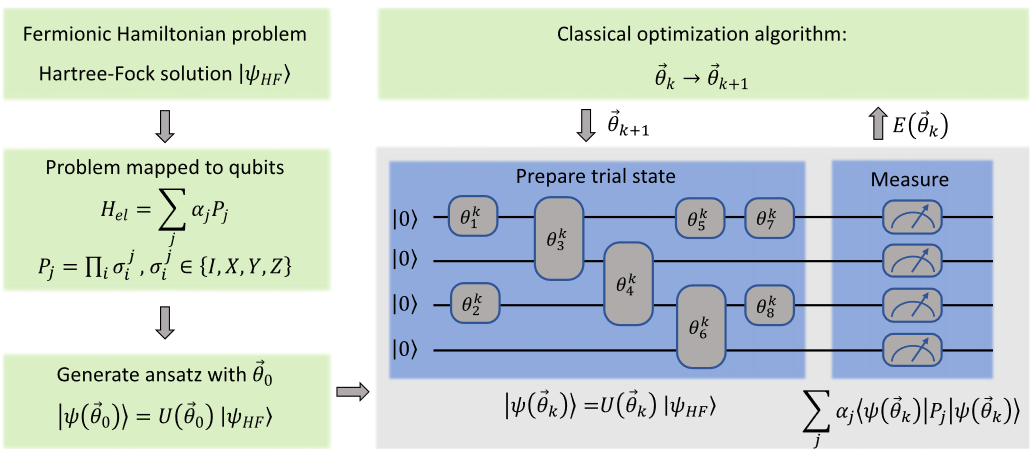
\includegraphics[width=0.8\textwidth]{figures/S3/flujovqe.png}
\caption{\label{fig:101} Flujo de trabajo del método \textit{variational quantum eigensolver}. Fuente: \cite{Fedorov2022}}
\end{figure}

\underline{\textit{Variational quantum deflation}}: 
La implementación del VQD sigue una estructura similar a la del VQE, con la diferencia que dentro del cálculo de la función de coste se considera un esquema de cálculo similar a la figura \ref{fig:102}. Para la función de coste ingresada se adapta para agregar el término de penalización, lo cual, agrega un coste adicional de listas para almacenar los parámetros de cada vector propio.

Para el cálculo del término de \textit{overlap} (penalización) se utiliza la expresión $U(\theta_k)U^{\dag}(\theta_i)$ con $i<k$, es decir, al \textit{ansatz} con los nuevos parámetros le añadimos el mismo \textit{ansatz} pero con la secuencia de términos invertidas y con los parámetros de uno de los estados anteriores. La idea es que, si volvemos al estado original, eso quiere decir que ambos estados son iguales y se tiene que penalizar.

La implementación solo puede ser utilizada en la combinación sistemas de espines con \textit{hardware efficient ansatz}.
\begin{figure}[H]
\centering
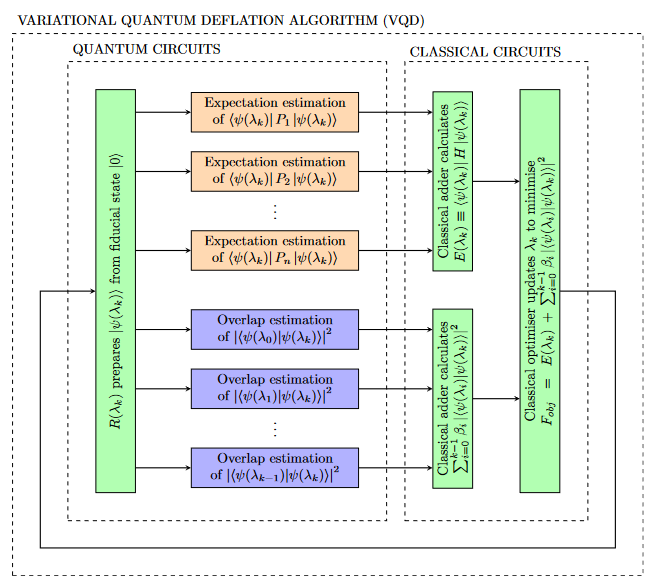
\includegraphics[width=0.75\textwidth]{figures/S3/flujovqd.png}
\caption{\label{fig:102} Flujo de trabajo del método \textit{variational quantum deflation}. Fuente: \cite{Higgott2019variationalquantum}}
\end{figure}




\subsubsection{Flujo de trabajo}
Finalmente, en esta última sección, se presentará un esquema general de los flujos de trabajo, junto con las subetapas. El flujo general se compone de 4 etapas, ver figura \ref{fig:110}, las cuales son independientes de los tipos de \textit{ansatz}, hamiltoniano, optimizador y método que se elijan. Cada una de estas etapas corresponde a la construcción de las tres clases mencionadas al inicio del capítulo, cada subetapa reflejas las operaciones que ocurren dentro de la clase y las que tienen que ser llamadas por el usuario.

\begin{figure}[H]
\centering
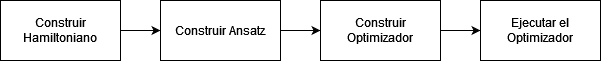
\includegraphics[width=0.8\textwidth]{figures/S3/flujogeneral.png}
\caption{\label{fig:110} Esquema general del flujo de trabajo. Fuente: Elaboración propia}
\end{figure}

La primera etapa está compuesta a su vez de 6 subetapas, ver figura \ref{fig:111}, la idea es un tipo de hamiltoniano y construirlo. Primero, se elige el tipo de hamiltoniano, ya que, de esa elección dependen los parámetros que se tienen que definir, una vez se tienen los parámetros, estos son utilizados para ejecutar funciones de las librerías que permiten construir los elementos básicos que son utilizados en la construcción de los hamiltonianos en el espacio de espines (en la representación propia de la librería), un detalle es que varias de las funciones utilizadas construyen términos de con constantes 0 (es decir, la constante que acompaña los términos es 0), por lo tanto, es menester aplicar un filtro que permite eliminar estos términos. Ahora que se tienen todos los términos, se utiliza la función para agrupar los términos conmutantes. Con lo anterior, tenemos un hamiltoniano expresado de una forma que nos permite realizar ejecuciones eficientes, los pasos siguientes consisten en reescribir estos grupos en la representación de lista de cadenas de Pauli y generar el representante de los grupos (este representante no es otra cosa que una cadena de caracteres, que nos indica que operador se encuentra en cada posición, este se utiliza para realizar los cambios de base correspondientes a cada \textit{qubit} a la hora de ejecutar los circuitos).

\begin{figure}[H]
\centering
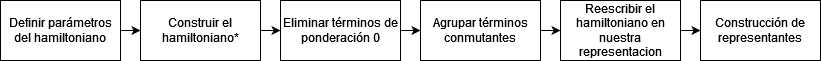
\includegraphics[width=0.99\textwidth]{figures/S3/flujo1.png}
\caption{\label{fig:111} Flujo de trabajo para construir el hamiltoniano del sistema. Fuente: Elaboración propia}
\end{figure}


La segunda etapa se compone de 4 subetapas, ver figura \ref{fig:112}, lo primero es definir los parámetros del \textit{ansatz}. Una vez hecho esto, se tiene que definir el \textit{backend} del \textit{ansatz} (el \textit{backend} contiene todas las configuraciones en las cuales se ejecutara el circuito), el siguiente es el simulador, en donde se ejecuta el circuito junto a las condiciones definidas \textit{backend} (modelos de ruido entre otros). Finalmente, el último elemento es el estado inicial del circuito, cabe mencionar, que este estado inicial no es el de los parámetros de las compuertas, es con el que se inicializa el circuito y al que después se le aplica el \textit{ansatz}.

\begin{figure}[H]
\centering
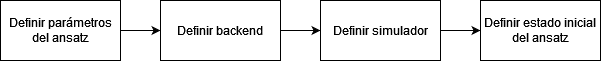
\includegraphics[width=0.9\textwidth]{figures/S3/flujo2.png}
\caption{\label{fig:112} Flujo de trabajo para construir el \textit{ansatz}. Fuente: Elaboración propia}
\end{figure}

La tercera etapa se compone de 3 subetapas, ver figura \ref{fig:113}, la idea de etapa es definir el optimizador que se va a utilizar para minimizar la función de coste. Entonces, lo primero es elegir el optimizador, uno de los optimizadores disponibles (ADAM y un método de gradiente genérico), en la práctica, los parámetros son los mismos para cada optimizador, por lo tanto, independiente de la selección, se tienen que definir los mismos parámetros. Una vez hecho esto, se construye la clase del optimizador.

\begin{figure}[H]
\centering
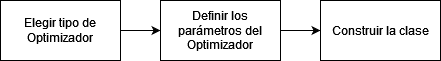
\includegraphics[width=0.7\textwidth]{figures/S3/flujo3.png}
\caption{\label{fig:113} Flujo de trabajo para construir el optimizador. Fuente: Elaboración propia}
\end{figure}

Finalmente, la cuarta etapa consiste en tomar la función de coste de la clase del hamiltoniano y ejecutar el optimizador (es decir, ejecutar el VQE o el VQD). Todo lo anterior es aplicable a cualquiera de las combinaciones que se definieron anteriormente, este flujo corresponde a un estándar para trabajar con los métodos variacionales cuánticos.


\newpage
\secnumbersection{VALIDACIÓN DE LA SOLUCIÓN}
En esta sección se presentarán los resultados obtenidos, comparando soluciones de otros métodos con las obtenidas de nuestro programa, además de hacer un análisis de recursos computacionales utilizados. Todos los cálculos de métodos variacionales cuánticos, fueron realizados utilizando el simulador \textit{default.qubit} y en condiciones sin ruido.


\subsection{Análisis de la relación hamiltoniano-\textit{ansatz}}
El objetivo de esta sección es el poder identificar regiones donde los \textit{ansazts} elegidos puedan capturar los estados de los hamiltonianos mientras variamos el valor de sus parámetros, ya que, es sabido que ciertas combinaciones de valores en los hamiltonianos pueden generar correlación mayor o menores, y es necesario saber si los \textit{ansatz} pueden o no capturarlas.

\subsubsection{Metodología}
Dado un hamiltoniano, elegimos uno de sus parámetros para analizar (en caso de tener más, los fijamos con valor arbitrario que no afecte el rendimiento). Luego se elige un conjunto de \textit{ansazt} que sean acordes al tipo de hamiltoniano. La idea es utilizar el VQE como una forma de poder analizar la relación hamiltoniano-\textit{ansatz}, ya que, si no es capaz de capturar el estado de mínima energía, es improbable que se pueda usar para métodos más avanzados (como el VQD)

Luego, para el optimizador, se utiliza un método de gradiente genérico con un \textit{learning rate} dé $0.3$. Los otros parámetros del optimizador van a ser informados en cada sección correspondiente. 

Entonces, se elige una cantidad $n$ de puntos del parámetro del hamiltoniano, para cada uno de estos se calcula el VQE $10$ veces para poder construir el promedio $\hat{x}$ y la desviación estándar $\sigma$ del valor de la energía en ese punto. Con estas dos cantidades podemos construir 3 casos en relación con el valor exacto del hamiltoniano con ese parámetro:
\begin{enumerate}
    \item Regiones de tipo 1: El valor exacto está dentro del intervalo $[\hat{x}-\sigma; \hat{x}+\sigma]$ y $|\sigma| \leq 10^{-6}$
    \item Regiones de tipo 2: El valor exacto está dentro del intervalo $[\hat{x}-\sigma; \hat{x}+\sigma]$ y $|\sigma| > 10^{-6}$
    \item Regiones de tipo 3: El valor exacto no pertenece al intervalo.
\end{enumerate}

Las regiones de tipo 1 corresponden a una situación idónea, donde las configuraciones iniciales permiten capturar de buena manera el estado de mínima energía. Las de tipo 2, muestra que, si bien es posible capturar el estado de mínima energía, uno de los hiperparámetros no es el adecuado para la tarea y este hace que se tenga una alta desviación estándar. Finalmente, las de tipo 3 se requiere un análisis un poco más detallado del porqué pareciera que el \textit{ansatz} no captura el estado. Para ello, se elige, sin pérdida de generalidad, un representante de la zona y se procede a hacer un análisis de algunos hiperparámetros para ver la razón del porqué genera esa diferencia. 


Los resultados exactos mostrados en la sección resultados, son calculados utilizando la rutina \textit{numpy.linalg.eigh} de la librería numpy para moléculas y modelos de espines, y la rutina  \textit{tenpy.algorithms.exact\_diag.ExactDiag} de la librería tenpy para los modelos de \textit{tight-binding} y Fermi-Hubbard.


\subsubsection{Definición de los sistemas}
\underline{Hamiltoniano de moléculas}: 
Para este hamiltoniano, se controlará el parámetro de distancia entre moléculas, se tendrá en consideración dos moléculas, un Hidruro de litio y un catión trihidrógeno. 


\begin{figure}[H]
\centering
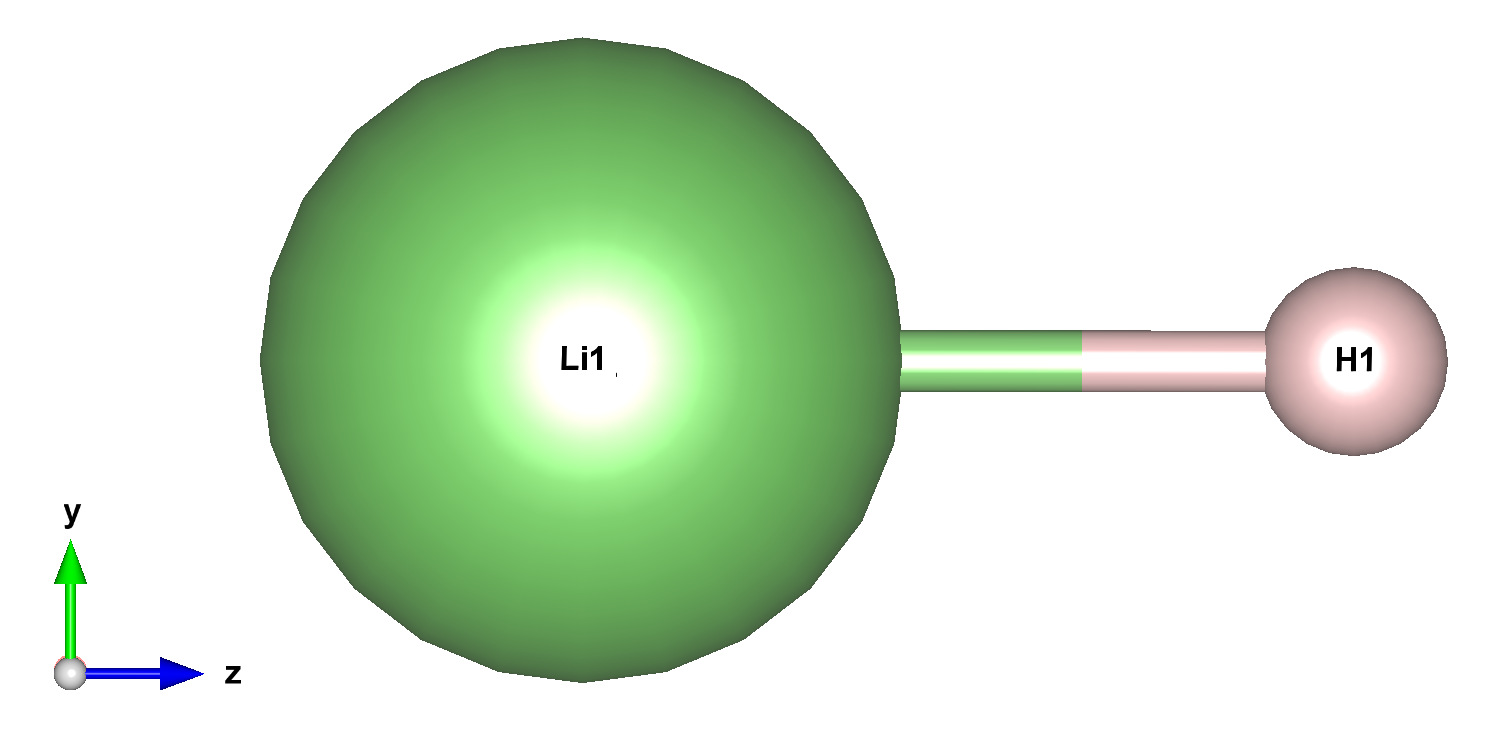
\includegraphics[width=0.5\textwidth]{figures/S4/moleculas/lih.png}
\caption{\label{fig:li} Hidruro de litio con una distancia de enlace por el eje Z. Fuente: Elaboración propia} 
\end{figure}

Para el hidruro de litio, ver figura \ref{fig:li}, se modela con los dos elementos desplazándose en el eje Z, se consideran 12 puntos del intervalo $[2;7]$, para el hamiltoniano se considera un espacio activo reducido, esto hace que el hamiltoniano se modele con 10 \textit{qubits} y 2 electrones. Por lo tanto, para el estado inicial, se considera un estado Hartree-fock de dos electrones ($\ket{1_11_20_3...0_{10}}$), el cual es utilizado en los \textit{ansatz} UCCSD y k-UpCCGSD (ambos con una repetición).

\begin{figure}[H]
\centering
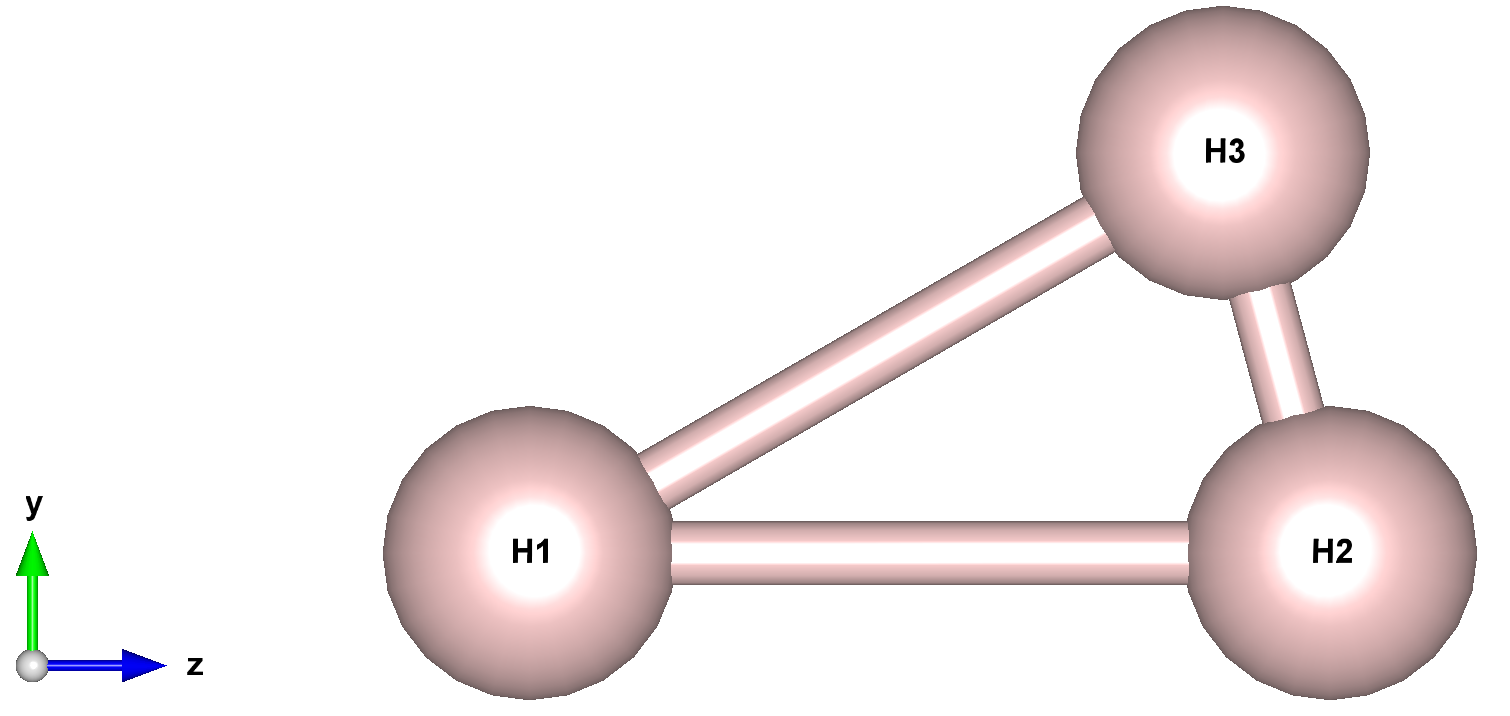
\includegraphics[width=0.5\textwidth]{figures/S4/moleculas/3h.png}
\caption{\label{fig:3h} Catión trihidrógeno modelado con un triángulo isósceles en el plano YZ. Fuente: Elaboración propia} 
\end{figure}

Para el catión trihidrógeno, ver figura \ref{fig:3h}, se modela como un triángulo isósceles en el plano YZ, se consideran 14 puntos del intervalo $[1.5; 8]$, para el hamiltoniano se considera un espacio activo completo con carga 1, ya que al ser un catión tiene un electrón menos, esto hace que el hamiltoniano se modele con 6 \textit{qubits} y 2 electrones. Para el estado inicial se considera un estado Hartree-fock de dos electrones ($\ket{1_11_20_3...0_{6}}$) que corresponde al número de electrones de valencia. Este estado inicial es utilizado en los \textit{ansatz} UCCSD y k-UpCCGSD (ambos con una repetición)

Para el optimizador, se consideran $60$ iteraciones máximas con una tolerancia dé $10^{-6}$.

\underline{Hamiltoniano de Fermi-Hubbard}: 
Para este hamiltoniano se consideran dos casos de interés, uno donde se controla el parámetro de \textit{hopping} $-t$ y otro donde se controla el parámetro de potencial $U$.

Para el primer caso, se consideraron 12 puntos del parámetro de \textit{hopping} $-t$ en el intervalo $[-1.5; 1.5]$ con un potencial $U=0$. Se consideraron los \textit{ansatz} UCCSD y k-UpCCGSD con una repetición, los cuales son inicializados en un estado Hartree-fock con un número de electrones igual a la cantidad de sitios (condición de \textit{half-filling}).

Para el segundo caso, el parámetro de \textit{hopping} se fija en el valor $-1$ y para el parámetro del potencial se consideran 6 puntos en el intervalo $[0;1]$. Se consideraron los \textit{ansatz} UCCSD y k-UpCCGSD con una repetición, los cuales son inicializados en un estado Hartree-fock con un número de electrones igual a la cantidad de sitios (condición de \textit{half-filling}).

Para ambos casos, se consideran sistemas de tamaños $3$ hasta $6$ y el optimizador tiene un límite de 100 iteraciones y una tolerancia dé $10^{-6}$.

\underline{Hamiltoniano de espín}: 
Para este hamiltoniano se controlará el parámetro $J$ usando un modelo XXX, el cual corresponde a un modelo donde todos los ejes tienen el mismo valor de \textit{exchange}. El parámetro $J$ puede tomar valores dentro de $[-1.5; 1.5]$ y se considerarán 13 puntos dentro del intervalo. 

Lo anterior va a hacer realizado en sistemas de $9$ a $12$ espines con condiciones abiertas y cerradas (una cadena y un anillo). Las ejecuciones van a ser llevadas a cabo considerando un estado inicial $\ket{0_10_2...0_{n-1}0_n}$, el \textit{ansatz hardware efficient} con una repetición. Para el optimizador, se consideran $100$ iteraciones máximas con una tolerancia dé $10^{-6}$.


\subsubsection{Resultados numéricos}
Considerando las condiciones antes expuestas, ahora se presentarán los resultados obtenidos para cada uno de los hamiltonianos.

\underline{Hamiltoniano de moléculas}:

\begin{figure}[H]
\centering
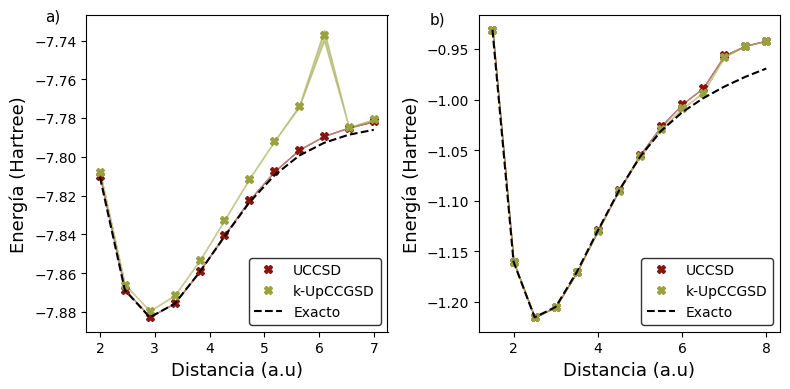
\includegraphics[width=0.9\textwidth]{figures/S4/moleculas/barridomoleculas.png}
\caption{\label{fig:5} VQE aplicado a a) $LiH$ y b) $H_3^{+}$ a distintas distancias entre moléculas. Fuente: Elaboración propia} 
\end{figure}

En la parte a) de la figura \ref{fig:5}, se puede ver como los mejores resultados se obtienen cerca del mínimo (es decir, en la distancia de equilibrio), al salir de esta región, se ve el \textit{ansatz} UCCSD presenta mejores resultados hasta donde ya el sistema se puede considerar dos moléculas aisladas. En el caso del k-UpCCGSD, se ve un aumento del error de forma considerable en zonas cercanas al mínimo, mostrando así un mal funcionamiento (alrededor de las $3.5$ (a.u)).

Pasando a la imagen b), vemos que ambos \textit{ansatz} presentan un buen rendimiento cerca del punto de equilibrio, solo cuando los hidrógenos están ya muy alejados entre sí, se ve un error perceptible. Esta mejora del k-UpCCGSD se puede explicar por la baja dimensionalidad del sistema.

Basándonos en que el UCCSD tiene un buen rendimiento en un rango amplio centrado en el punto de equilibrio, no es necesario realizar un análisis, ya que, es raro estudiar moléculas tan alejadas del mínimo. Por otro lado, si tomaremos el k-UpCCGSD para ver el porqué de la diferencia en el mínimo de la molécula $LiH$ (constituye una región del tipo 2). Dicho esto, consideraremos la distancia de equilibrio de $2.969280527$ (a.u) ($5.5822473$ (ángstrom)) para el \textit{basis set} ''sto-3g'' indicada en la CCCBD \cite{CCCBDB}. 


En la figura \ref{fig:10}, se puede el efecto de aplicar repeticiones al \textit{ansatz} (además de modificar el \textit{learning rate} a $0.2$ y aumentar el número de iteraciones a 100), en ninguno de los casos se ve una mejora sustancial de la solución, observando la gráfica del error se ve que después de la caída abrupta el error empieza a decaer muy lentamente, hasta las 100 iteraciones, no se ve ningún estancamiento que permita generar conclusiones respecto al \textit{ansatz}. Pero, como requiere tantas iteraciones, esto nos indica que no es un \textit{ansatz} adecuado para esta molécula. 

\begin{figure}[H]
\centering
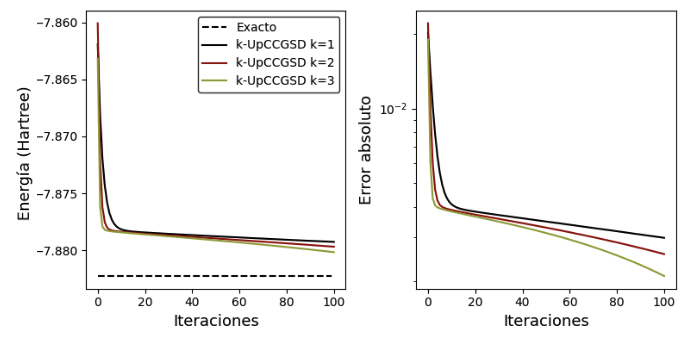
\includegraphics[width=0.9\textwidth]{figures/S4/moleculas/barridomoleculas2.png}
\caption{\label{fig:10} VQE aplicado a $LiH$ con diferentes repeticiones. Fuente: Elaboración propia}
\end{figure}


\underline{Hamiltoniano de Fermi-Hubbard}:

En la figura \ref{fig:6}, se puede observar el comportamiento del VQE sobre el modelo de \textit{tight binding}. Partiendo con el \textit{ansatz} UCCSD, se ve que este es capaz de capturar sin problemas las correlaciones independientes del tamaño y condiciones de borde, aunque para valores pequeños de $t$, se ven pequeñas diferencias respecto al valor exacto. Luego, si pasamos al \textit{ansatz} k-UpCCGSD, tenemos una situación similar, con la diferencia que para valores $|t|>1$, el \textit{ansatz} da malos resultados (ver cadena de 6 sitios), pero para valores menores a 1, presenta un rendimiento similar al UCCSD.

\begin{figure}[H]
\centering
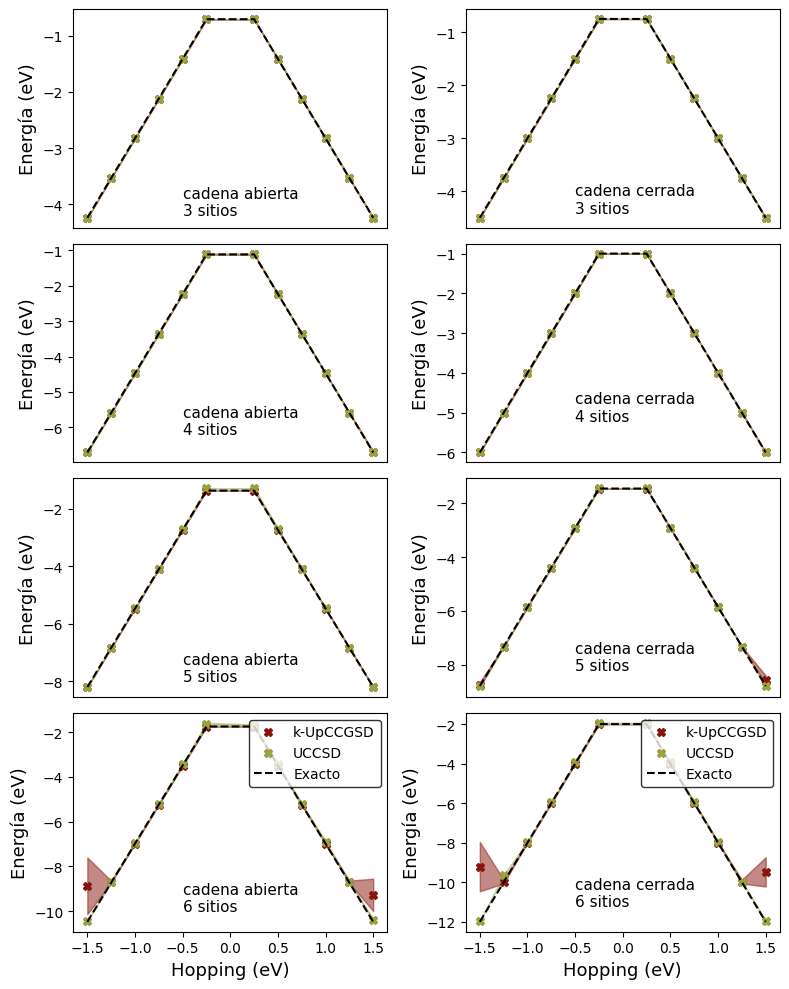
\includegraphics[width=0.8\textwidth]{figures/S4/tb/barridotb.png}
\caption{\label{fig:6} VQE aplicado a diferentes valores de $t$ con $U=0$ (\textit{tight biding}). Fuente: Elaboración propia}
\end{figure}

Para factores prácticos, nos es útil que se tenga un buen rendimiento para valores $t=1$, ya que, en la práctica, es común cocientar el hamiltoniano para que el término de \textit{hopping} sea igual a 1 (pero esto es solo posible, si él $t$ es el mismo para cada sitio, lo cual puede variar en algunas ocasiones). Es por ello por lo que, en vez de concentrarnos sobre el error en los valores grandes, nos concentraremos en el error en los valores cercanos a 0. Dicho esto, sin pérdida de generalidad, tomaremos una cadena de 5 sitios con condiciones de borde abiertas y un \textit{hopping} $t=0.15$, para este análisis solo consideraremos el \textit{ansatz} UCCSD (ya que este es el que presenta diferencias sustanciales al valor exacto). Como no es posible aplicar repeticiones a esta \textit{ansatz}, se estudiarán otros hiperparámetros.

\begin{figure}[H]
\centering
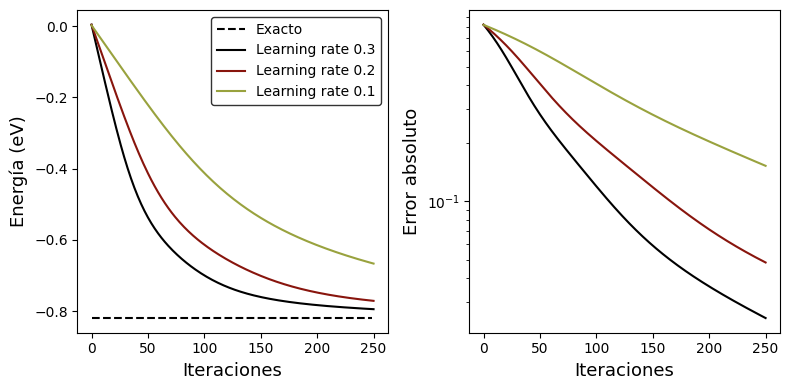
\includegraphics[width=0.9\textwidth]{figures/S4/tb/barridotb2.png}
\caption{\label{fig:11} VQE aplicado al modelo \textit{tight binding} con $t=0.15$. Fuente: Elaboración propia}
\end{figure}

En la figura \ref{fig:11} se pueden ver los efectos de modificar el \textit{learning rate} del optimizador, en ninguno de los casos se ve una mejora sustancial, lo cual nos indica que el \textit{ansatz} con una sola repetición no es capaz de capturar el estado de mínima energía cuando él $|t|<< 1$.

\begin{figure}[H]
\centering
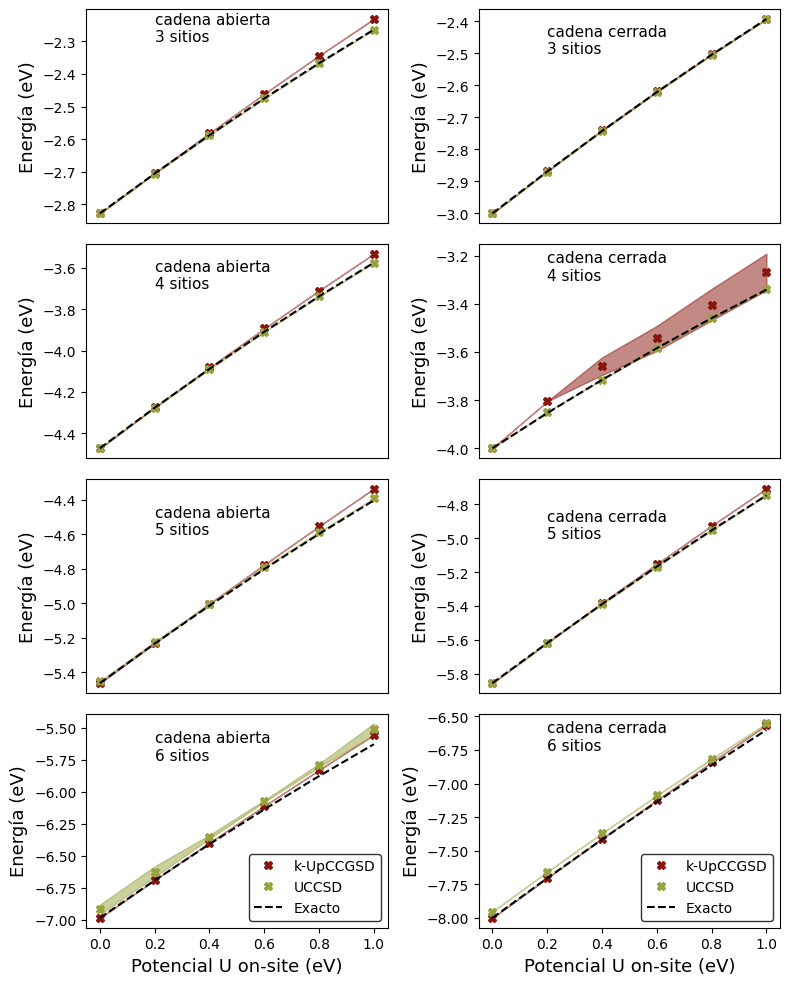
\includegraphics[width=0.9\textwidth]{figures/S4/fermi/barridofh.png}
\caption{\label{fig:7} VQE aplicado a diferentes valores de $U$ con $t=1$ (Fermi-Hubbard). Fuente: Elaboración propia}
\end{figure}

Pasando al modelo de Fermi-Hubbard, con $t=1$, encontramos un resumen de los valores obtenidos en la figura \ref{fig:7}. De esta imagen se puede observar cómo los mejores resultados se obtienen del \textit{ansatz}  k-UpCCGSD dentro de un intervalo entre 0.0 y 0.4 aproximadamente (ignorando el caso con 4 sitios y condiciones de borde cerrada), fuera de este rango, se ve como las curvas se empiezan a separar de la línea del valor exacto.

Cuando vamos aumentando el tamaño del sistema, se observa como el UCCSD va dando soluciones peores en contraste al otro \textit{ansatz} (esto, dentro y fuera del rango mencionado en el párrafo anterior), independiente de las condiciones de borde y del valor del potencial. A continuación, analizaremos el caso particular de k-UpCCGSD para 4 sitios en la cadena cerrada para el valor de $U=0.4$, y para el UCCSD consideraremos el caso de 6 sitios con condiciones de borde abierta y un valor dé $U=0.0$.

\begin{figure}[H]
\centering
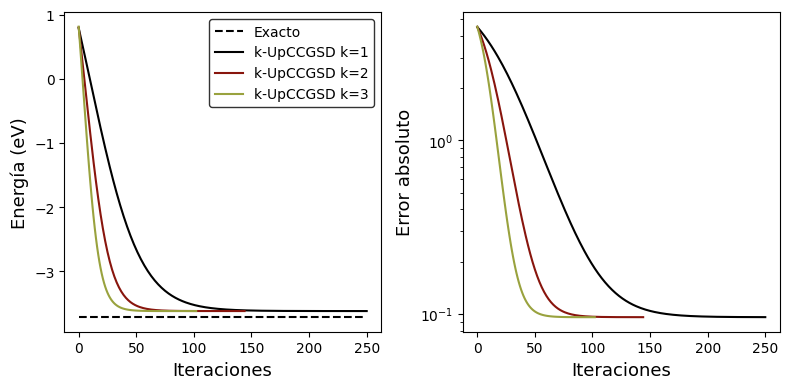
\includegraphics[width=0.9\textwidth]{figures/S4/fermi/barridofh2.png}
\caption{\label{fig:12} VQE aplicado al modelo de Fermi-Hubbard de 4 sitios con condiciones de borde cerradas con $t=1$ y $U=0.4$ y \textit{ansatz} k-UpCCGSD. Fuente: Elaboración propia}
\end{figure}

En la figura \ref{fig:12} se puede observar como a pesar de aumentar el número de repeticiones (además de aumentar el número de iteraciones a 250 y disminuir el \textit{learning rate} a $0.01$) del \textit{ansatz}, no se ve una mejora sustancial en el error, solo se aprecia una convergencia más rápida al mínimo que el \textit{ansazt} puede calcular (cantidad que varía del valor exacto). Viendo este comportamiento, es posible indicar que este \textit{ansatz} para ese caso particular, no es el adecuado, existe una incapacidad del \textit{ansatz} para capturar correctamente el estado de mínima energía.

\begin{figure}[H]
\centering
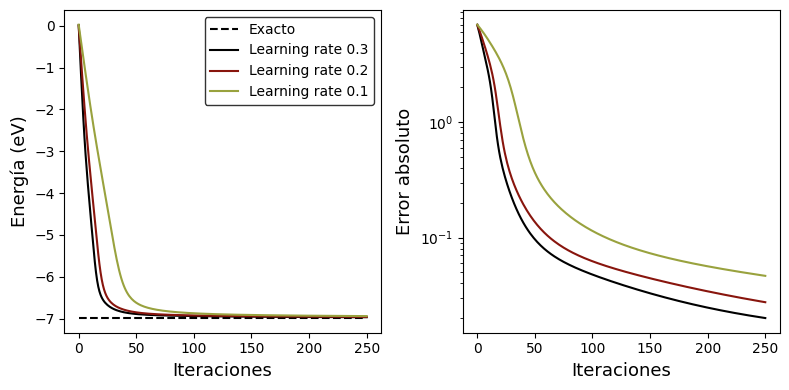
\includegraphics[width=0.9\textwidth]{figures/S4/fermi/barridofh3.png}
\caption{\label{fig:13} VQE aplicado al modelo de Fermi-Hubbard de 6 sitios con condiciones de borde abiertas con $t=1$ y $U=0.0$, y \textit{ansatz} UCCSD. Fuente: Elaboración propia}
\end{figure}

Ahora, pasando al siguiente caso, en la figura \ref{fig:13} se puede observar los efectos de la variación del \textit{learning rate} (además de aumentar el número de iteraciones a 250) sobre el cálculo del estado de mínima energía. En ninguno de los casos se observa una mejora sustancial, solo mediante el aumento del número de iteraciones se ve como el error absoluto va disminuyendo, pero esto genera problemas de viabilidad por el alto número de iteraciones requeridas para alcanzar el error buscado. Es por ello por lo que se puede indicar que este \textit{ansazt} no es el adecuado para este sistema cuando el número de sitios aumenta.

\underline{Hamiltoniano de espín}: 
En la figura \ref{fig:1}, se puede observar los resultados obtenidos para sistemas de distinto tamaño y de diferentes condiciones de borde, mientras se varía el \textit{exchange} $J$. Uno de los detalles que se observa a simple vista es para valores positivos de \textit{exchange} se observan valores que solapan el valor exacto y tienen una desviación de estándar menor que la tolerancia (región de tipo 1). Mientras que para valores negativos se observa, de manera preliminar, que el promedio no captura el valor exacto, además de tener desviaciones estándar por sobre la tolerancia (región de tipo 3). Ambas situaciones parecen ser independientes del tamaño y de las condiciones de borde.

\begin{figure}[H]
\centering
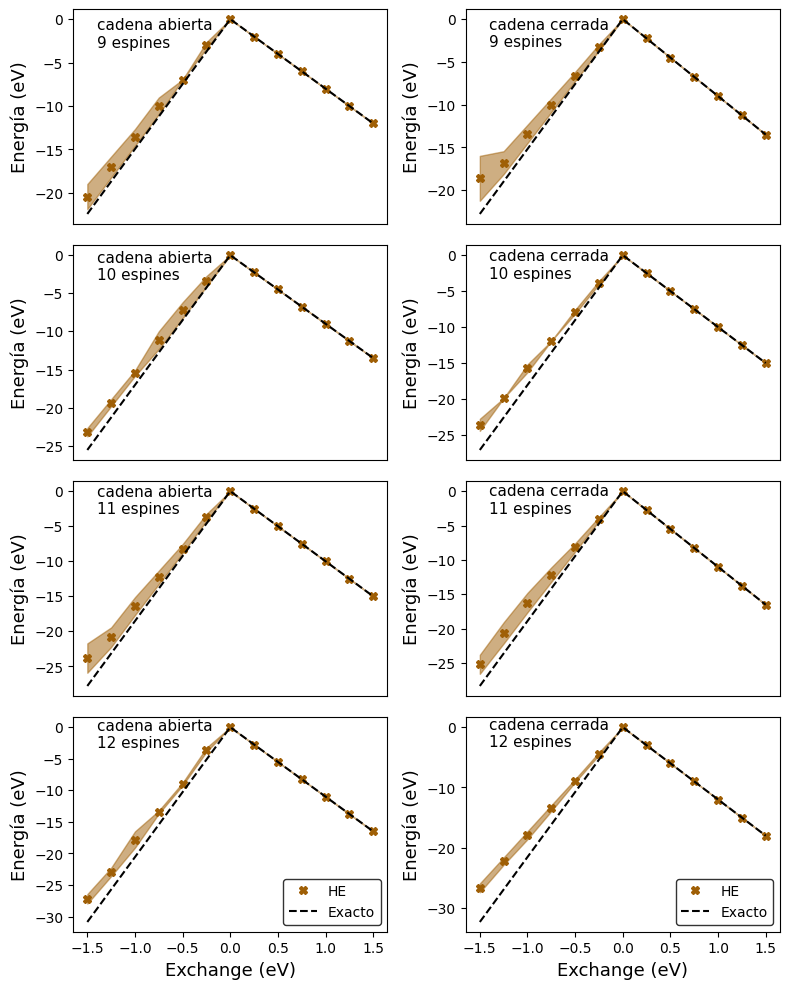
\includegraphics[width=0.9\textwidth]{figures/S4/spins/barridoespines.png}
\caption{\label{fig:1} VQE aplicado la modelo de espines a diferentes valores de $J$. Fuente: Elaboración propia}
\end{figure}

Dicho lo anterior, los valores positivos corresponden a una región de tipo 1, mientras que los valores negativos corresponden a una de tipo 3, por lo tanto, es necesario realizar un análisis más detallado para este tipo de valores.

Entonces, sin pérdida de generalidad, se toma una cadena abierta de 9 espines con un valor de \textit{exchange} $J=-1$ (eV) (modelo XXX). En la figura \ref{fig:8} se puede observar la convergencia del VQE a medida que aumentamos las repeticiones del \textit{ansatz} para alcanzar correlaciones más complejas, a pesar de esto, en la gráfica del error absoluto se ve como ninguna de estas parece alcanzar una rápida convergencia, además de mostrar síntomas de estancamiento a medida que aumentamos el número de iteraciones.

\begin{figure}[H]
\centering
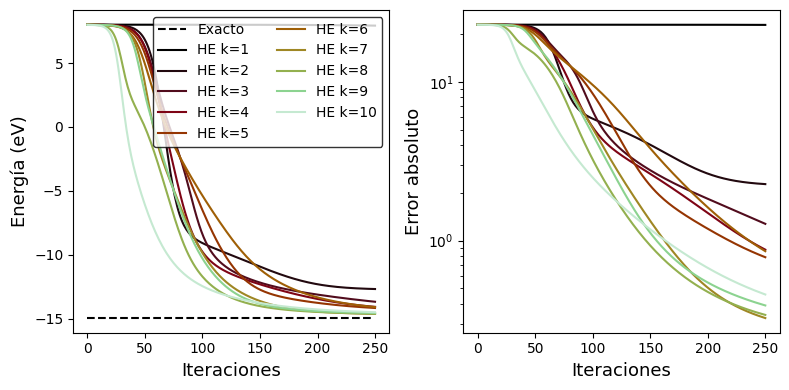
\includegraphics[width=0.9\textwidth]{figures/S4/spins/barridoespines2.png}
\caption{\label{fig:8} VQE aplicado al modelo de espines considerando 9 espines con $J=-1$ (eV) y condiciones de borde abierta. Acá se consideran 250 iteraciones y un \textit{learning rate} de $0.01$. Fuente: Elaboración propia}
\end{figure}

\begin{figure}[H]
\centering
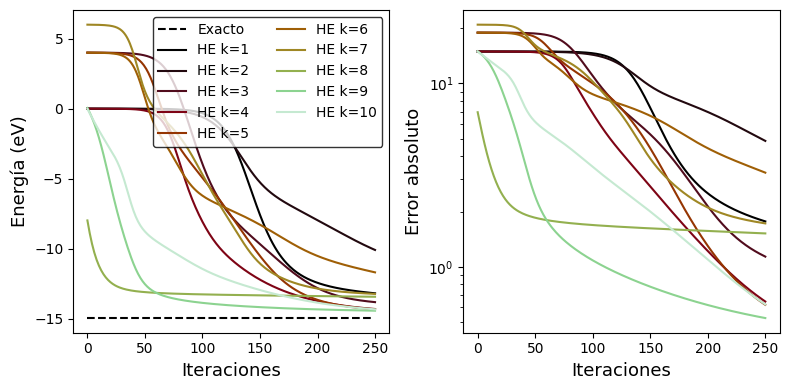
\includegraphics[width=0.9\textwidth]{figures/S4/spins/barridoespines3.png}
\caption{\label{fig:9} VQE aplicado al modelo de espines considerando 9 espines con $J=-1$ (eV) y condiciones de borde abierta. Acá se consideran 250 iteraciones, un \textit{learning rate} de $0.01$ y un estado inicial $\ket{010101010}$. Fuente: Elaboración propia}
\end{figure}

En consideración que al variar estos parámetros no hay ninguna mejora, lo otro que se tiene que probar es el punto inicial, en la figura \ref{fig:9} se puede ver los efectos del cambio inicial, pero, a pesar de ello, ninguno muestra una tendencia de la cual se puede esperar que alcance la tolerancia buscada. Por lo tanto, acá se puede concluir que el problema es la capacidad del \textit{ansatz} de capturar el estado de mínima energía, ya que, la otra opción es aumentar el número de repeticiones, lo cual puede llegar a ser muy costoso.













%%
%%
%%
%%
\subsection{Análisis de uso de memoria}
En esta sección, lo que se busca es el poder comparar de forma cuantitativa el uso de memoria que puede requerir el almacenamiento del hamiltoniano utilizando diferentes técnicas de representación. Como acá estamos comparando requerimientos de memoria, se eligen valores arbitrarios para los parámetros del hamiltoniano.

\subsubsection{Metodología}
En esta sección se busca comparan 4 representaciones posibles de un hamiltoniano, una matricial, otra en listas de cadenas de Pauli, otra en MPS/MPO y finalmente la representación que utilizan por defecto en Pennylane.

Para la matricial, se calculará de forma teórica el uso de memoria, considerando que cada elemento de esta es un número de 8 \textit{bytes} (\textit{float64}). Para la representación de MPO, utilizaremos la librería de python tenpy que implementa las redes tensoriales que son utilizadas para la construcción MPS, MPO y ejecución de DMRG. 

Para las representaciones de MPO, de Pennylane y la de listas de cadenas de Pauli, se utilizará la función \textit{asizeof} de la librería de python pympler. La idea es analizar el crecimiento de uso de memoria a medida que aumentamos el tamaño del sistema.

Por temas de notación, ''pennylane'' hace referencia a la representación de Pennylane, ''tenpy'' hace referencia a la representación MPS/MPO, ''matriz'' hace referencia al cálculo antes mencionado y ''nuestra clase'' hace referencia a la lista de cadenas de Pauli.

\subsubsection{Definición de los sistemas}

\underline{Hamiltoniano de moléculas}:
Para este hamiltoniano, se considerarán dímeros de elementos entre el hidrógeno y el nitrógeno, estos hamiltonianos son construidos utilizando todo el espacio activo, considerando el \textit{basis set} sto-3g. Todos estos dímeros son construidos considerando una distancia de $1.5$ (a.u) entre los átomos.

Para este hamiltoniano se considerarán tres representaciones, la representación matricial, la representación de Pennylane y la representación en lista de cadenas de Pauli. No se tiene en cuenta la representación MPS/MPO porque esta no tiene una implementación directa para moléculas, es por ello por lo que se decidió no utilizarla, ya que se escapa de los alcances de la memoria.

\underline{Hamiltoniano de Fermi-Hubbard}:
Para este hamiltoniano, se consideran dos casos, el primero es considerando valores $t=1$ y $U=0.0$, el segundo es con valores $t=1$ y $U=2.0$ (el primero caso corresponde al modelo \textit{tight biding} y el segundo corresponde al modelo Fermi-Hubbard). En ambos casos, se tiene una estructura de anillo, ya que esta tiene más términos que una cadena y sirve como una cota superior para sistemas de cadenas.

Para este hamiltoniano se considerarán cuatro representaciones, la representación matricial, la representación de Pennylane, la representación en MPS/MPO y la representación en lista de cadenas de Pauli.

\underline{Hamiltoniano de espín}: 
Para este hamiltoniano, se considera un modelo de espines XXX (mismo \textit{exchange} para todos los ejes) con un valor $J=1$ (eV). Al igual que para el hamiltoniano anterior, se considera una estructura de anillo.

Para este hamiltoniano se considerarán cuatro representaciones, la representación matricial, la representación de Pennylane, la representación en MPS/MPO y la representación en lista de cadenas de Pauli.


\subsubsection{Resultados de uso de memoria}
\underline{Hamiltoniano de moléculas}:

\begin{figure}[H]
\centering
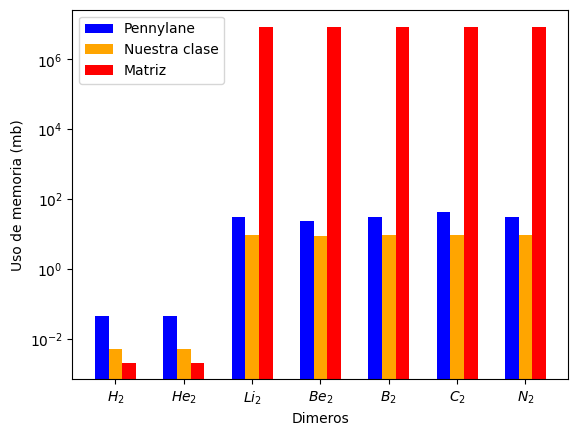
\includegraphics[width=0.7\textwidth]{figures/S4/moleculas/usomemoriamols.png}
\caption{\label{fig:20} Uso de memoria de los diferentes hamiltonianos de dímeros en (mb). Fuente: Elaboración propia}
\end{figure}

En la figura \ref{fig:20} se puede observar la diferencia de requerimientos de memoria que cada hamiltoniano necesita para almacenarse en una variable durante los flujos de cálculo. Para sistemas de baja dimensionalidad ($H_2$ y $He_2$ que requieren 4 \textit{qubits}), las matrices son menos costosa que las otras representaciones, pero cuando pasamos a sistemas más grandes, se aprecia una clara diferencia, donde nuestra representación y la de Pennylane ofrecen un uso más eficiente de recursos. Entre ambas, la diferencia no es muy sustancial, pero nuestra representación ofrece un uso de memoria menor.

En ninguno de los casos se observa una tendencia, ya que los hamiltonianos están a base de los orbitales que tienen cada elemento, por lo tanto, para establecer un flujo se tendría que seleccionar sistemas que tengan diferentes consideraciones de orbitales.



\underline{Hamiltoniano de Fermi-Hubbard/\textit{tight binding}}:

\begin{figure}[H]
\centering
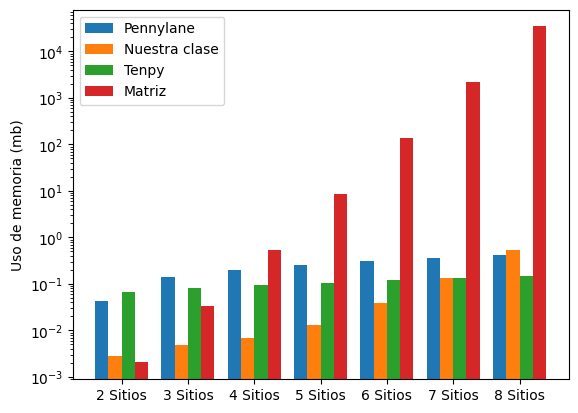
\includegraphics[width=0.7\textwidth]{figures/S4/tb/usomemoriatb.png}
\caption{\label{fig:21} Uso de memoria del hamiltoniano \textit{tight binding} a diferente número de sitios en (mb). Fuente: Elaboración propia}
\end{figure}


Para el caso del modelo de \textit{tight binding}, podemos visualizar en la figura \ref{fig:21}, los costos de memoria asociados a mantener el hamiltoniano almacenado en el flujo. En comparación a almacenar la matriz completa, las otras representaciones muestran un consumo menor. Si concentramos el análisis en las tres representaciones, vemos que tanto tenpy como Pennylane ofrecen una representación con consumos similares, en contraste con la nuestra, para menos de 8 sitios se ve una mejora, mientras que, para más de 8 sitios, nuestra representación muestra un consumo superior, pero no es una diferencia sustancial. 

La representación matricial muestra una tendencia lineal, considerando que la escala de la gráfica es logarítmica, mientras que Pennylane y tenpy muestran tendencias logarítmicas. Finalmente, nuestra representación tiene una tendencia que parece una mezcla entre lineal y exponencial, pero, para poder hablar de una forma más certera, se requiere aumentar la cantidad de sitios.

\begin{figure}[H]
\centering
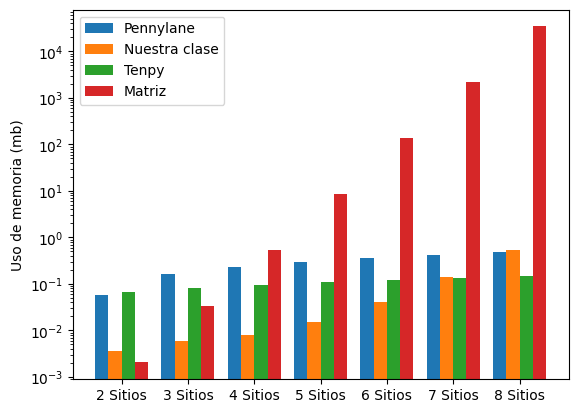
\includegraphics[width=0.7\textwidth]{figures/S4/fermi/usomemoriafh.png}
\caption{\label{fig:22} Uso de memoria del hamiltoniano Fermi-Hubbard a diferente número de sitios en (mb). Fuente: Elaboración propia}
\end{figure}


Ahora, pasando al modelo de Fermi-Hubbard, el resumen de costos se puede observar en la figura \ref{fig:22}. Como el modelo de Fermi-Hubbard es esencia, el modelo de \textit{tight biding} con unos cuantos términos extras, la tendencia es similar. Las representaciones de Pennylane y tenpy ofrecen rendimientos similares, que, en contraste con la nuestra, están muy cercanas.


\underline{Hamiltoniano de espín}:
Para el caso del modelo de espines XXX, el resumen de costos se puede observar en la figura \ref{fig:23}. Al igual que en los sistemas anteriores, la representación matricial es la que más recursos utiliza. Dejando está de lado, las representaciones de Pennylane y tenpy ofrecen un consumo considerablemente inferior a la matricial. Finalmente, nuestra representación ofrece un consumo inferior a las anteriores mencionadas, pero a medida que aumenta el número de espines esta es muy cercana al consumo de Pennylane y tenpy. Al igual que con los modelos anteriores, se aprecia como nuestra representación muestra tendencias entre lineales y exponenciales.


\begin{figure}[H]
\centering
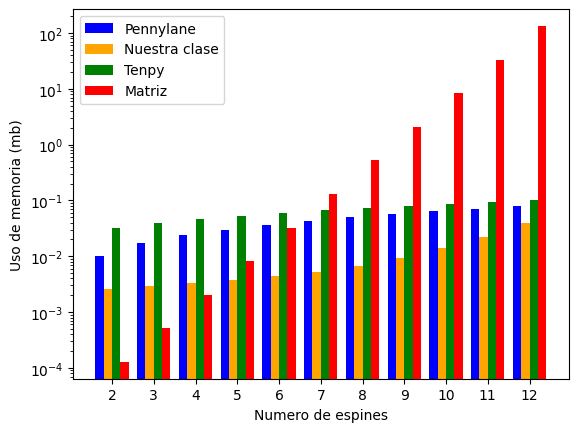
\includegraphics[width=0.7\textwidth]{figures/S4/spins/usomemoriahei.png}
\caption{\label{fig:23} Uso de memoria del hamiltoniano de espines XXX a diferente número de espines en (mb). Fuente: Elaboración propia}
\end{figure}

%%
%%
%%
\subsection{Análisis de tiempos}
El siguiente tema por tratar es el análisis de los tiempos de cómputo. Los cálculos que se muestran a continuación fueron realizados en un \textit{mac mini} con un \textit{chip Apple M2 Pro} con 32 GB de memoria Ram y 10 \textit{cores}, este dispositivo pertenece al grupo de simulaciones del departamento de física USM.

Dentro de este contexto, diagonalización exacta debe entenderse como el proceso de obtención de valores y vectores propios, para este caso utilizamos la rutina de la librería numpy \textit{numpy.linalg.eigh} que calcula estas cantidades de una matriz hermitiana. Para la DMRG, utilizamos la rutina \textit{tenpy.algorithms.dmrg.TwoSiteDMRGEngine} de la librería tenpy.


\subsubsection{Metodología}
Para cada hamiltoniano se elegirá valores de zonas de tipo 1, ya que en estas se tiene asegurada una convergencia ''rápida'' y una solución muy cercana al valor exacto. De esta forma podemos comparar el rendimiento de una forma justa. De trabajar en otras zonas, es claro que el tiempo está dado por el límite de iteraciones, lo cual no es lo que se busca. Es necesario mencionar que el tiempo considerado es desde el momento de ejecución del optimizador (para ejecutar el VQE) y las rutinas mencionadas anteriormente (de DMRG y diagonalización exacta) hasta finalizan, acá no se toma en cuenta el tiempo tomado en construir el hamiltoniano.

Los optimizadores serán informados dependiendo de cada caso, pero todos van a ser fijados con 100 iteraciones máximas y una tolerancia de $10^{-6}$, el resto de parámetros serán informados en cada hamiltoniano.

Finalmente, todos los cálculos son realizados utilizando CPU y con un solo proceso (no hay paralelización implementada, además del \textit{broadcasting} propio de numpy).

\subsubsection{Definición de los sistemas}

\underline{Hamiltoniano de moléculas}: 
Para el hamiltoniano molecular, se utilizará un arreglo 1D de hidrógenos, es decir, se van colocando hidrógenos en el eje Z, a una distancia de $1.3228$ (a.u) ($2.486864$ (angstrom)) entre cada uno, formando así la estructura 1D. Para este, se considera el \textit{basis set} ''sto-3g'', el \textit{ansatz} elegido es el UCCSD, ya que, basándonos en el análisis de la sección hamiltoniano-\textit{ansatz}, es el que mejor resultados da a medida que el sistema crece. Para el optimizador, se utilizará el gradiente genérico con \textit{learning rate} dé $0.3$.


\underline{Hamiltoniano de Fermi-Hubbard}: 
Del análisis de la sección hamiltoniano-\textit{ansatz} tenemos dos casos de interés, el primero es considerando $t=1$ y $U=0.0$ (\textit{tight binding}) y el segundo es $t=1$ y $U=0.2$ (Fermi-Hubbard), en ambos casos, se considerará en \textit{ansatz} k-UpCCGSD, y un optimizador genérico con \textit{learning rate} de $0.3$


\underline{Hamiltoniano de espín}: 
Del análisis de la sección hamiltoniano-\textit{ansatz} se elige un modelo XXX con una estructura de cadena, el valor del \textit{exchange} es dé $1.25$. El \textit{ansatz} que se utiliza es el \textit{hardware efficient} con una repetición. El optimizador elegido es un gradiente genérico con un \textit{learning rate} dé $0.3$.


\subsubsection{Resultados de tiempo de cómputo}

\underline{Hamiltoniano de moléculas}: 
\begin{figure}[H]
\centering
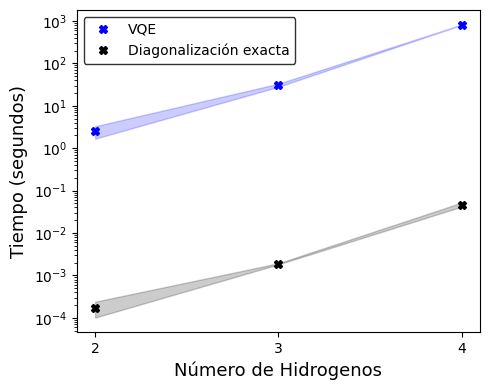
\includegraphics[width=0.7\textwidth]{figures/S4/moleculas/tiempomoleculas.png}
\caption{\label{fig:33} Tiempos de cómputo del estado de mínima energía en cadenas 1D de hidrógeno en segundos. Fuente: Elaboración propia}
\end{figure}

En la figura \ref{fig:33}, se puede observar el comportamiento de los tiempos de cómputo a medida que aumentamos el número de hidrógenos en la cadena. Si bien se tienen pocos puntos, se puede apreciar como ambos tiempos se comportan como líneas rectas paralelas (en escala logarítmica), en las cuales, el VQE tarda más que la diagonalización exacta.

Si entramos dentro de un análisis más detallado, encontramos que a medida que aumentamos el tamaño, el VQE requiere más ejecuciones ($5$, $16$, $67$ respectivamente), y el número de parámetros también aumenta ($3$, $8$, $26$ respectivamente).


\underline{Hamiltoniano de Fermi-Hubbard}: 
\begin{figure}[H]
\centering
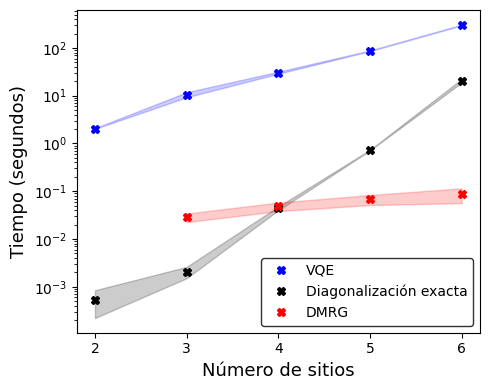
\includegraphics[width=0.7\textwidth]{figures/S4/tb/tiempotb.png}
\caption{\label{fig:34} Tiempos de cómputo del estado de mínima energía en el modelo de \textit{tight binding} en segundos. Fuente: Elaboración propia}
\end{figure}

En la figura \ref{fig:34} se puede ver el comportamiento de los tiempos de cómputo a medida que aumentamos el número de sitios en el modelo de \textit{tight binding}. El VQE se muestra como el que más tiempo tarda, con una tendencia lineal a medida que crece el sistema, por otro lado, la diagonalización exacta muestra tiempos menores, pero con una tendencia exponencial. Finalmente, DRMG muestra los mejores tiempos cuando crece el sistema con una tendencia logarítmica (recordando que el gráfico está en escala logarítmica). 

Para el VQE, se tiene que independiente del número de sitios, el circuito se tiene que ejecutar cuatro veces por llamada de la función de coste, y a medida que crece el sistema, el número de parámetros es $6$, $18$, $36$, $60$ y $90$ respectivamente.


\begin{figure}[H]
\centering
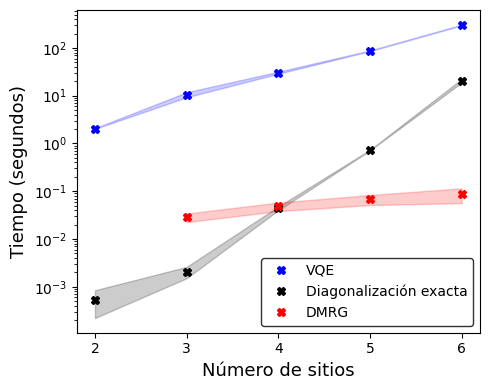
\includegraphics[width=0.7\textwidth]{figures/S4/fermi/tiempofb.png}
\caption{\label{fig:35} Tiempos de cómputo del estado de mínima energía en el modelo de Fermi-Hubbard en segundos. Fuente: Elaboración propia}
\end{figure}

Ahora, pasando al modelo de Fermi-Hubbard, ver figura \ref{fig:35}, tenemos comportamientos similares, ya que, en esencia ambos modelos son muy similares, solo se agregan nuevos términos. En temas de tiempo de ejecución, no existen diferencias sustanciales.

Si entramos a analizar el VQE, encontramos que el número de ejecuciones pasa a cinco y el número de parámetros se mantiene igual al de \textit{tight binding}.

\underline{Hamiltoniano de espín}: 

\begin{figure}[H]
\centering
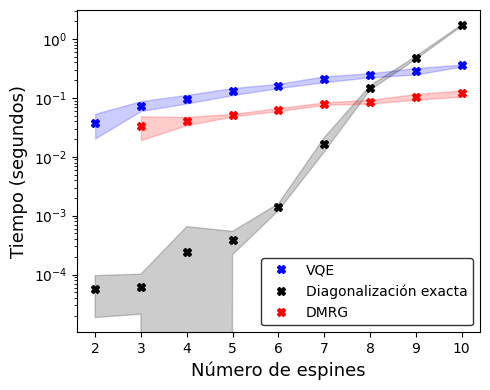
\includegraphics[width=0.7\textwidth]{figures/S4/spins/tiempoespines.png}
\caption{\label{fig:36} Tiempos de cómputo del estado de mínima energía en el modelo de Heisenberg en segundos. Fuente: Elaboración propia}
\end{figure}

Ahora, pasando al modelo de espines, ver figura \ref{fig:36}, tenemos nuevamente que el VQE es el que más tarda para sistemas de baja dimensionalidad, pero en sistemas de mediana dimensionalidad (sobre 8 espines), se ve que es mejor que la diagonalización exacta. El VQE muestra una tendencia entre lineal y logarítmica, mientras que diagonalización exacta tiene una tendencia que parece exponencial. Luego tenemos DMRG que tiene un comportamiento paralelo que el VQE, con la diferencia que ofrece tiempos menores.

Al igual que en el modelo anterior, el número de ejecuciones del circuito por cómputo de la función de coste es constante (tres ejecuciones), mientras que el número de parámetros si crece al aumentar el tamaño, este tiene un crecimiento lineal respecto al número de espines.







%%
%%
%%
%%
\subsection{Más allá del VQE}
En esta sección, el objetivo es realizar estudios más complejos utilizando el VQE, de manera más concreta, nos enfocaremos en dos tópicos, el primero es dinámica molecular en el sentido de relajación de estructuras y el segundo es simular los efectos de la temperatura en alguna estructura.

Respecto al primer tópico, la idea es colocar una molécula donde los elementos no están en sus respectivas distancias de equilibrio, y desde ese punto, utilizando el VQE, poder simular el movimiento molecular que permite que los átomos se muevan a sus distancias de equilibrio \cite{OptimizationStruture}.

Para el segundo tópico, la idea es poder realizar termodinámica usando ordenadores cuánticos utilizando algunos de los métodos definidos, para ello se busca calcular los todos los niveles de energía del sistema para poder calcular de forma clásica, semi clásica los efectos de la temperatura sobre algún observable como la magnetización o el calor especifico. 

Es importante destacar que acá no se busca analizar el uso de recursos (tiempo y memoria), acá solo nos interesa la calidad de ciertos valores de interés, los cuales serán indicados más adelante dependiendo del tópico.

\subsubsection{Metodología}
El objetivo de esta sección es proponer una metodología para poder llevar a cabo estudios de una forma metódica y estándar que permita comparar resultados de buena calidad.

Lo primero es el elegir los hiperparámetros adecuados (el \textit{ansatz} y el optimizador), entonces, dado un sistema, lo primero es elegir un conjunto de \textit{ansatzs} adecuados (que por el contexto tengan sentido utilizarlos), para comparar la capacidad del \textit{ansatz} utilizaremos el VQE con un optimizador genérico con configuraciones base y con un número distinto de repeticiones. La razón detrás de esto es que si el \textit{ansatz} no es capaz de capturar el estado de mínima energía, no va a ser capaz de capturar otras características. 

Una vez elegido el \textit{ansatz} lo siguiente es elegir el mejor optimizador basándonos en este \textit{ansatz}, como los pasos de optimización son costosos, el criterio de selección es a base de la tolerancia obtenida contra el número de pasos (en este caso, se prueban diferentes métodos y diferentes \textit{learning rates} si es que corresponde). Sobre la base de esto, es que podemos discriminar el mejor par de \textit{ansatz} y optimizador para el sistema y trabajar en las mejores condiciones.


Para la metodología del primer tópico, como se están trabajando con moléculas, la idea es elegir un estado cercano al mínimo ($\pm 0.3$ (ángstrom) de la distancia de equilibrio), ya que, por cómo se vio en la sección de ''Análisis de la relación hamiltoniano-\textit{ansatz}'' los \textit{ansatz} para moléculas tienen un buen funcionamiento cercano a la distancia de equilibrio. Para este tópico, se requieren dos optimizadores, uno para los parámetros del \textit{ansatz} y otro que va a representar el movimiento por el espacio (acercando o alejando los elementos). Como acá estamos dejando la molécula ''libre'', tenemos que repetir esta ejecución 10 veces para poder construir un promedio y una desviación estándar representativa, de esta forma se podrá comparar con el valor de distancia real, cabe mencionar, que acá no nos interesa tanto la calidad de la solución de la energía nos interesa la distancia molecular.

Ahora pensando a la metodología del segundo tópico, este se puede entender como un proceso de dos pasos, el primero es el poder capturar todos los niveles de energía y el segundo es el estimar la distribución de probabilidad de los estados. 

Para el primer caso, vamos a seguir el mismo procedimiento que el utilizado para las regiones de tipo 1, primero vamos a ver cuántas repeticiones del \textit{hardware efficient ansatz} se necesitan para capturar el estado de mínima energía, acá buscamos el número máximo de repeticiones que se puede seleccionar hasta que no se vea mejora (como el objetivo es capturar estados excitados, no podemos esperar que el \textit{ansatz} que captura el estado de mínima energía sea suficiente para capturar los excitados). Una vez seleccionado el número de repeticiones, podemos pasar a calcular los niveles excitados usando el VQD, acá vamos a repetir este cálculo 10 para tener un conjunto que represente la viabilidad a la hora de ejecutar el VQD. 

Para el segundo paso, vamos a utilizar cada una de las 10 repeticiones para construir la distribución de estados y calcular el calor especifico (generando así 10 distribuciones y 10 curvas de calor especifico). Esta distribución de estados se calcula de forma clásica calculando el producto $\exp{-E_i/k_b t}/\mathcal{Z}$ (siendo $E_i$ las energías obtenidas del VQD). La idea, es que estos resultados se comparen con los obtenidos de forma exacta (calculando los valores y vectores propios usando diagonalización exacta).

%El estudiante realizo una tesis en un area de frontera, de manera interdiciplinaria entre las ciencias computacionales y la física-química, en un campo recientemente abierto al mundo. Creo que debe publicarse.

\subsubsection{Definición de los sistemas}

\begin{figure}[H]
\centering
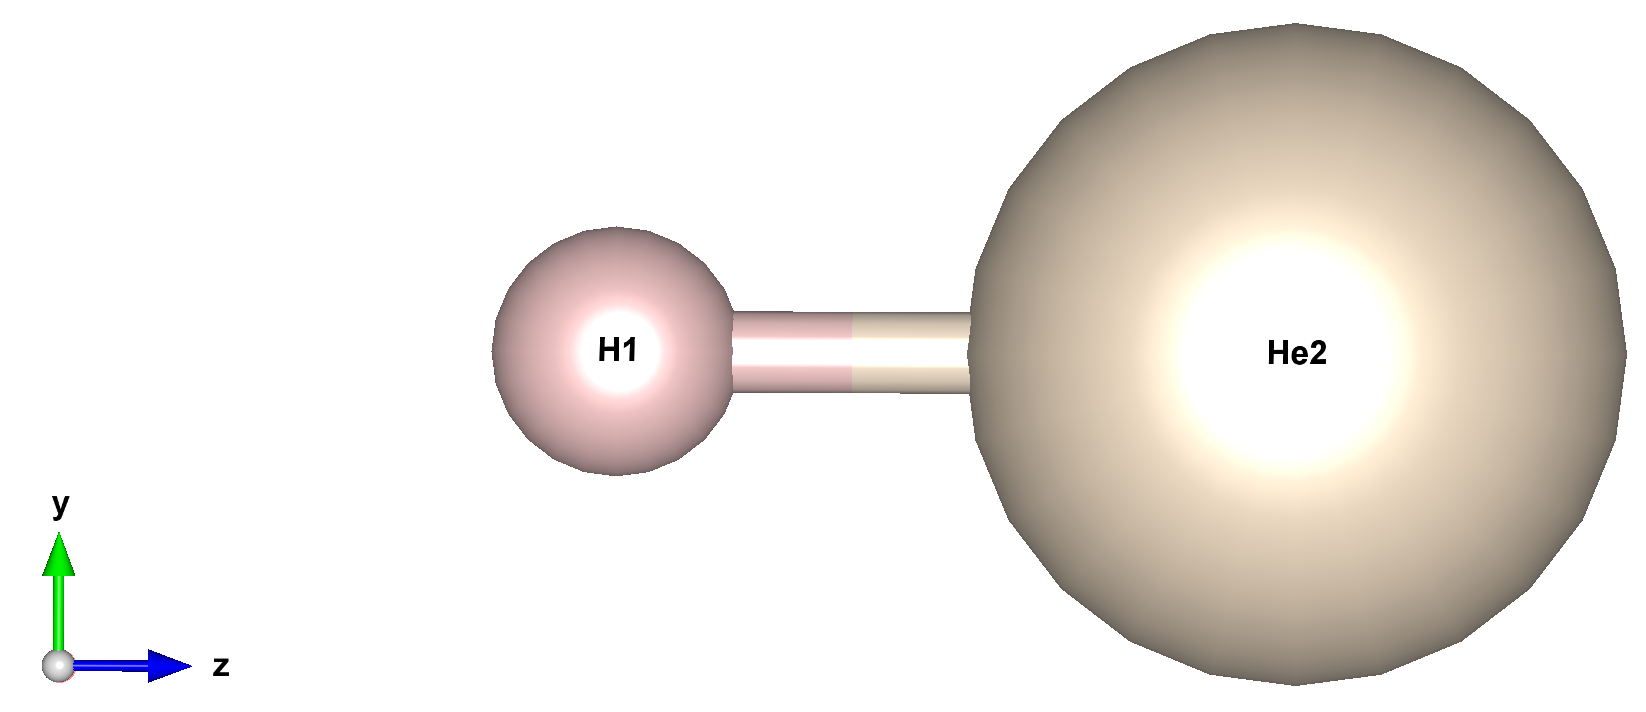
\includegraphics[width=0.5\textwidth]{figures/S4/moleculas/hhe.png}
\caption{\label{fig:hhe} Ion de helio hidrógeno con una distancia de enlace por el eje Z. Fuente: Elaboración propia}
\end{figure}


Para la optimización de las distancias, se tomará como sistema el ion de helio hidrógeno, ver figura \ref{fig:hhe}, este será construido usando el \textit{basis set} ''sto-3g'' a una distancia de $0.6$ (ángstrom) en el eje Z. Utilizando la CCCBDB \cite{CCCBDB}, sabemos que la distancia en equilibrio usando este \textit{basis set} es de $0.9295$ (ángstrom).

Para el análisis de temperatura, consideramos un modelo de espines XXX con 3 espines, con condiciones de borde abiertas y un \textit{exchange} $J = 1.0$ (eV).

\subsubsection{Resultados numéricos}

\underline{Optimización de estructuras}:
Comenzando con el ion de helio hidrógeno, este se puede considerar como un sistema de baja dimensionalidad (el espacio es más pequeño que el catión trihidrógeno), por lo tanto, considerando lo visto en la sección de '’Análisis de la relación hamiltoniano-\textit{ansatz}'', ambos \textit{ansatz} (UCCSD y k-UpCCGSD) van a tener un buen rendimiento. Dicho la elección del \textit{ansatz} pasa a ser algo más arbitrario, en este caso, se trabajará con el UCCSD (que fue el que mejor resultados dio para el catión trihidrógeno). Para el optimizador de los parámetros del \textit{ansatz} se usará el optimizador genérico con un \textit{learning rate} fijo dé $0.2$. 

\begin{figure}[H]
\centering
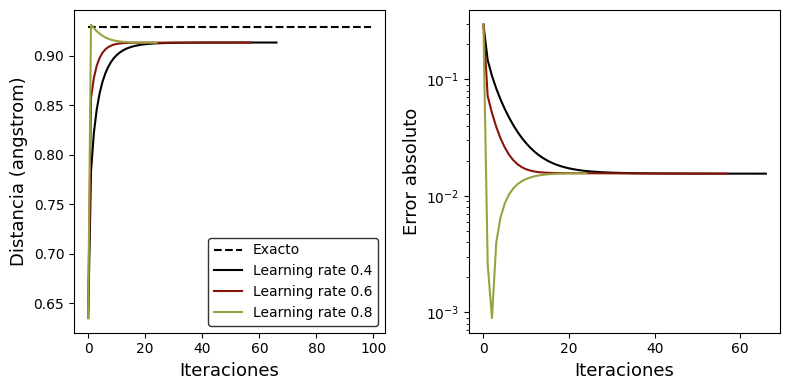
\includegraphics[width=0.8\textwidth]{figures/S4/moleculas/estructuras1.png}
\caption{\label{fig:41} VQE aplicado a cálculo de distancia molecular utilizando un optimizador genérico. Fuente: Elaboración propia}
\end{figure}

En la figura \ref{fig:42} se puede observar los resultados de con optimizador genérico con diferentes \textit{learning rates}. En ninguno de los casos, se observa que se alcance la distancia real, a pesar de la anomalía con el \textit{learning rate} $0.8$. Frente a esto, se cambia el optimizador por ADAM con un nuevo conjunto de \textit{learning rates} más pequeños (esto también implica que tengamos que aumentar el número de iteraciones máximas).

\begin{figure}[H]
\centering
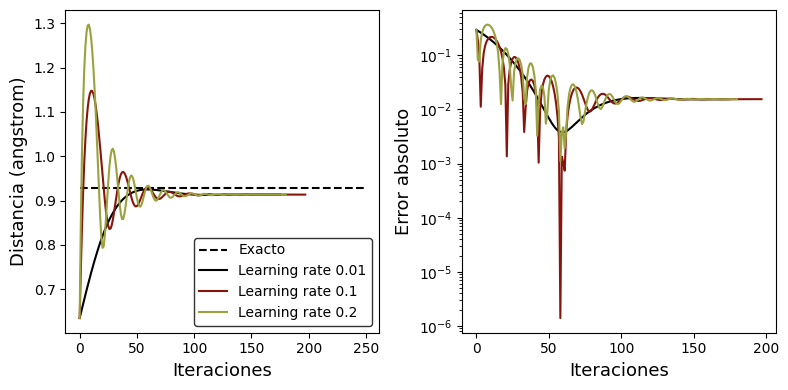
\includegraphics[width=0.8\textwidth]{figures/S4/moleculas/estructuras2.png}
\caption{\label{fig:42} VQE aplicado a cálculo de distancia molecular utilizando el optimizador ADAM. Fuente: Elaboración propia}
\end{figure}


Los efectos del optimizador se puede observar en la figura \ref{fig:42}, donde se pueden observar resultados similares a los obtenidos con el gradiente genérico, a pesar de la anomalía que se observa con el \textit{learning rate} $0.1$. Frente a esto, nos quedaremos con el gradiente genérico con \textit{learning rate} $0.6$ que nos entrega resultados similares en menor número de iteraciones.


\begin{figure}[H]
\centering
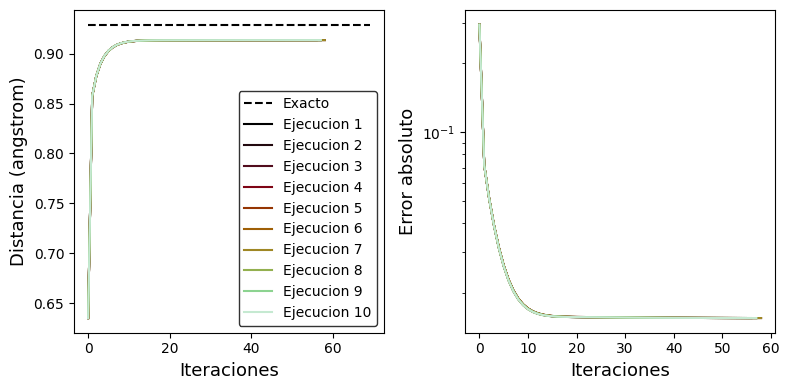
\includegraphics[width=0.8\textwidth]{figures/S4/moleculas/estructuradistancia.png}
\caption{\label{fig:43} VQE aplicado a cálculo de distancia molecular utilizando los mejores hiperparámetros. Fuente: Elaboración propia}
\end{figure}

\begin{figure}[H]
\centering
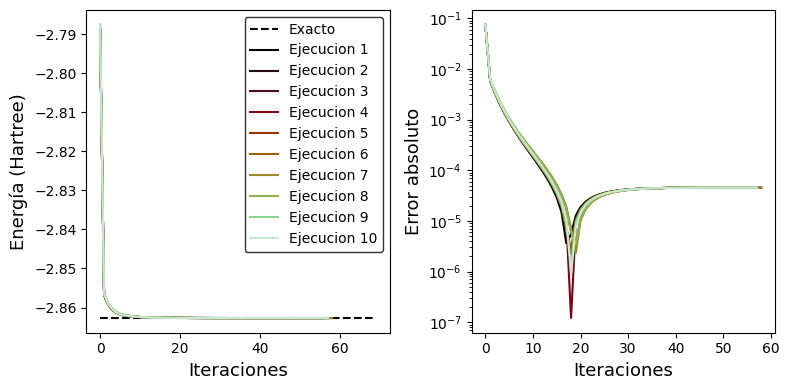
\includegraphics[width=0.8\textwidth]{figures/S4/moleculas/estructuraenergia.png}
\caption{\label{fig:44} VQE aplicado a cálculo de energía del estado de mínima energía utilizando los mejores hiperparámetros. Fuente: Elaboración propia}
\end{figure}


Dicho lo anterior, ahora que tenemos definidos los hiperparámetros, podemos analizar los resultados del sistema, las figuras \ref{fig:43} y \ref{fig:44} se puede observar la convergía de las diversas repeticiones en la energía y distancia del sistema respectivamente. En estas dos figuras se puede observar los efectos de la baja dimensionalidad (hay poca variabilidad entre ejecuciones), por otro lado, se observa una anomalía en el error absoluto de la energía obtenida (ver figura \ref{fig:44}) cerca de las 15 iteraciones, lo cual puede ser explicado como un efecto colateral de la convergencia de las distancias entre elementos. Por otro lado, si nos centramos en la figura \ref{fig:43}, es posible apreciar cómo no se alcanza la distancia de equilibrio, el error se estanca en un error absoluto de alrededor $10^{-1}$. 


\underline{Niveles excitados y temperatura}: 
Ahora respecto al sistema de espines, como acá estamos buscando capturar todos los niveles excitados, primero se tiene que hacer un análisis de las repeticiones del \textit{ansatz} para obtener la mayor cantidad posible de tal forma de poder asegurar que el \textit{ansatz} es capaz de capturar estados excitados. 

\begin{figure}[H]
\centering
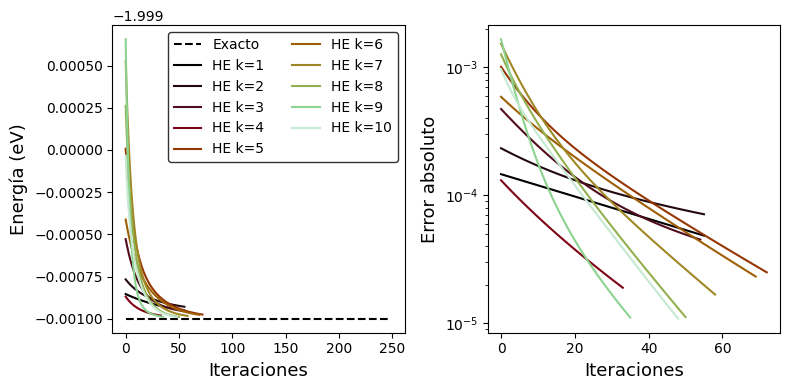
\includegraphics[width=0.8\textwidth]{figures/S4/spins/temperatura1.png}
\caption{\label{fig:45} VQE aplicado a modelo de espines considerando 3 espines con condiciones de borde abiertas. Fuente: Elaboración propia}
\end{figure}

En la figura \ref{fig:45} se puede observar el efecto de aumentar el número de repeticiones (para no tener efectos de oscilaciones en la convergencia, acá se redujo el \textit{learning rate} a $0.01$ y se aumentó el número de iteraciones a 250), en todos los casos se observa una convergencia, el error se reduce de manera casi lineal en escala logarítmica. Para este caso, nos quedaremos con 10 repeticiones para asegurar una buena captura de estados excitados.

\begin{figure}[H]
\centering
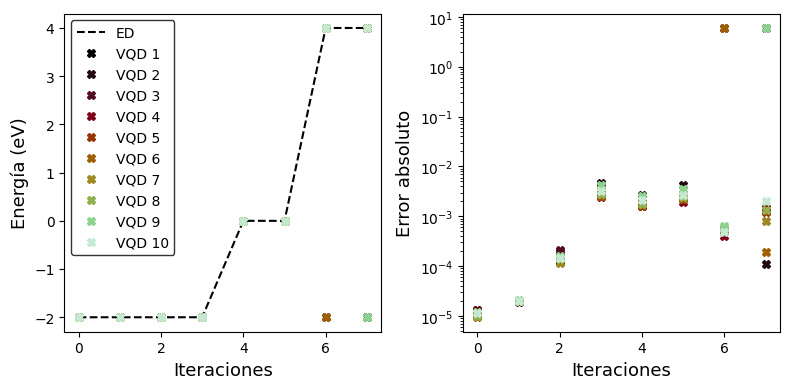
\includegraphics[width=0.8\textwidth]{figures/S4/spins/temperatura2.png}
\caption{\label{fig:46} VQD aplicado a modelo de Heisenberg de 3 espines con condiciones de borde abiertas. Fuente: Elaboración propia}
\end{figure}

Dicho lo anterior, nos quedaremos los hiperparámetros mencionados anteriormente para ejecutar el VQD. En la figura \ref{fig:46} se puede observar un resumen de los niveles obtenidos en las 10 ejecuciones del VQD. En varias ejecuciones se ve como se obtienen niveles erróneos que escapan del valor exacto (también se ve en la gráfica del error, donde en un par de casos llega a un error cercano a $10^{1}$), pero en general, se observa una buena captura de los estados excitados en las ejecuciones.

Visto que en gran parte de los casos el VQD funciona bien, podemos pasar a hablar de la estimación de la distribución de estados. Acá la idea es utilizar un enfoque híbrido para el cómputo de la distribución, donde se utilizan las energías obtenidas del VQD para calcular las exponenciales correspondientes. Acá consideraremos el conjunto de $[1, 2, 4, 8, 16, 32]$ (K) para calcular el calor especifico.

\begin{figure}[H]
\centering
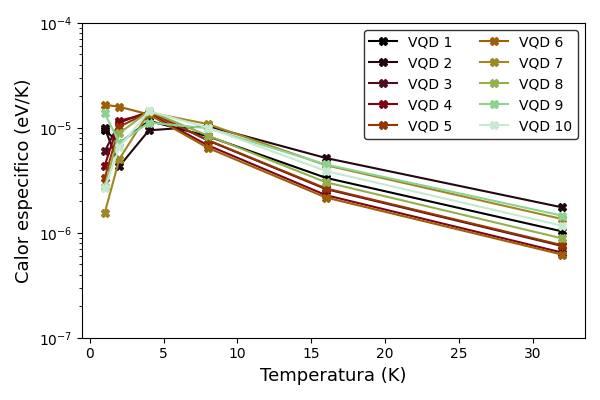
\includegraphics[width=0.8\textwidth]{figures/S4/spins/temperatura3.png}
\caption{\label{fig:47} Calor especificó calculado usando energías obtenidas del VQD. Fuente: Elaboración propia}
\end{figure}

En la figura \ref{fig:47} se puede observar el cálculo del calor específico para cada una de las ejecuciones del VQD, en la mayoría de los casos se observa un pequeño máximo para luego empezar a decaer. Esta cantidad no puede ser comparada con valores exactos por una indeterminación de las operaciones (algunos cálculos de exponenciales sufren de \textit{overflow} considerando \textit{float128}, haciendo que todos los valores sean retornados sean 0). Frente a esto, se tienen dos posibles conclusiones, respecto al fenómeno, se ve que se obtienen tendencias que son esperadas (cambios de fases) por efectos de las temperaturas, también podemos analizar respecto a su cercanía al valor 0, dentro de lo cual, estamos dentro de una tolerancia aceptable.

Independiente de esto, se puede observar como técnicas como el VQD nos pueden ser útil a la hora de tratar de estudiar observables termodinámicos.


\newpage
\secnumbersection{CONCLUSIONES}
El presente capítulo se estructura en cuatro secciones, el primer subcapítulo se concentra en proporcionar visión general de los resultados obtenidos en el capítulo 4. En el segundo subcapítulo se analiza cómo los resultados se vinculan con el cumplimiento de los objetivos y en el tercero se presenta una perspectiva sobre el trabajo pendiente, el futuro y las mejoras. El último subcapítulo corresponde a las palabras finales del autor, sobre todo el proceso de desarrollo y el producto final.

\subsection{Visión general de los resultados}
Como en el capítulo 4 se analizan diversos aspectos, vamos a dirigirnos subcapítulo por subcapítulo, dando unas cuantas palabras acerca de los resultados alcanzados.

En capítulo 4.1 se evidenció, en varias situaciones, la importancia de la elección de \textit{ansazt} para asegurar resultados con un bajo error. La situación más clara se presenta en la figura \ref{fig:1}, en la cual, para un mismo \textit{ansazt}, los efectos de la elección del parámetro $J$ afectan de forma notable en los valores numéricos de las soluciones obtenidas. Después hay otro problema cuando dos \textit{ansazt}, generados de la teoría \textit{Unitary couple cluster}, no representan la misma física. Esto es visible en la figura \ref{fig:5}, donde para la molécula de $LiH$, los \textit{ansazt} UCCSD y kUpCCGSD dan resultados distintos. Esto evidencia lo sensible del tema de la elección de \textit{ansazt}, donde la única solución aparente es realizar los cálculos con un conjunto de \textit{ansazt}.

En el capítulo 4.2, se observaron las diferencias en el consumo de memoria RAM de cada una de las presentaciones, respectivamente. Dejando de lado los dímeros de elementos, se visualizó una tendencia de nuestra representación (presentada en el capítulo 3.2.2), a medida que el sistema aumentaba en tamaño, que solo compite con las otras representaciones consideradas en sistemas de tamaño pequeño a mediano, ya para sistemas de mayor tamaño, teniendo en cuentas las tendencias mostradas, se requerirá una mayor cantidad de memoria. Esto hace que sea necesario replantear la implementación de nuestra representación para hacerlo más eficiente en sistemas de mayor tamaño.

En el capítulo 4.3, se puede ver que el VQE es el que más tiempo necesita. En la figura \ref{fig:36}, se ve mejor que Diagonalización exacta y una tendencia que parece logarítmica (considerando que el eje Y está en escala logarítmica). Estos resultados hacen que sea necesario replantear la implementación realizada además de los \textit{ansazt} seleccionados, ya que, son estos los que determinan el número de parámetros que el optimizador debe manejar.

Finalmente, el capítulo 4.4 fue un experimento para probar posibles extensiones del VQE que permiten ser aplicados para realizar otro tipo de cálculos, el primero de ellos una relajación estructural, cuyo objetivo es llevar a los elementos de una molécula a su estado de equilibrio, en las figuras \ref{fig:41} y \ref{fig:42} se puede ver como distintos optimizadores lograron alcanzar distancias con un error final de $10^{-2}$, lamentablemente este error sigue siendo considerable, teniendo en cuenta que estamos en unidades ángstrom. El segundo experimento fue para calcular observables termodinámicos utilizando el VQD para obtener los niveles excitados, en la figura \ref{fig:46} se puede ver en promedio, los resultados obtenidos son concordantes con los valores exactos, a pesar de que en algunos casos el método falla en las predicciones. Estos errores tienen sus repercusiones en los cálculos siguientes. En ambas aplicaciones se puede apreciar su potencial, no obstante, es necesario dedicar un mayor desarrollo para alcanzar resultados más satisfactorios.

Con todo lo anterior se puede mencionar que los resultados no son los esperados, en las diferentes gráficas se puede ver como el VQE presenta un peor rendimiento en contraste con los otros, por otro lado, la representación de los hamiltonianos elegida muestra tendencias que denotan que no es útil para estructuras grandes. No obstante, las curvas de tendencia del VQE presentan un gran potencial si se implementa de una forma más sofisticada (por ejemplo, mediante paralelización).


%
%
%
%
%
\subsection{Análisis sobre los objetivos}
Con lo expresado en el subcapítulo anterior, podemos pasar a hablar sobre como el desarrollo presentado en el capítulo 4 refleja un \textbf{cumplimiento} de los objetivos presentados en los capítulos 1.3.1 y 1.3.2.

\subsubsection{Primer objetivo específico}
El primer objetivo se define como ''Realizar un estudio que muestre los requerimientos de almacenamiento de los modelos de tipo Fermi-Hubbard, \textit{tight binding}, Heisenberg y estructuras moleculares''. Este estudio se lleva a cabo en el capítulo 4.2, en donde se definen las cuatro posibles representaciones en que se pueden escribir estos modelos (matricial, redes tensoriales, lista de cadenas de Pauli y la representación propia de la librería). Considerando estas cuatro opciones, se utiliza una función de una librería especialidad para estudiar el consumo de memoria de variables (Pymbler), el capítulo 4.2.3 se presentan los resultados que muestran cuanta memoria RAM requieren las variables a medida que aumentamos el tamaño del sistema, de estas gráficas, se pueden derivan las diversas tendencias de cada representación. Esta información nos es útil para determinar en qué forma tenemos que representan los modelos de tal forma que podamos mantener un uso de memoria mínimo.

\subsubsection{Segundo objetivo específico}
El tercer objetivo se define como ''Realizar un \textit{benchmark} que contraste los tiempos de ejecución y el error absoluto asociado a la solución obtenida, para el problema de valores y vectores propios, de un algoritmo clásico-exacto, clásico-variacional y variacional cuántico, considerando los modelos expuestos en el punto 1''.

Este \textit{benchmark} se encuentra reflejado en los capítulos 4.1 y 4.3. En el primero de ellos se estudia un problema importante que es la relación hamiltoniano-\textit{ansazt}, mostrando la cercanía de la solución obtenida con la solución exacta (a pesar de que el error absoluto de la convergencia solo se muestra para puntos concretos). En este estudio no solo se varían los parámetros del hamiltoniano, sino que, sé varía también el tamaño, pasando de sistemas de baja a mediada dimensionalidad. 

Respecto al segundo capítulo, como solo se trabajan con valores del hamiltoniano que se sabe que funcionan bien, el tema de la calidad de la solución es obviada para solo concentrar el análisis en los tiempos a medida que se aumenta el tamaño del sistema. En este se pueden visualizar las tendencias que presenta cada método en los diferentes modelos, viendo desde tendencias logarítmicas hasta lineales en una escala logarítmica.

Este \textit{benchmark} no considera todos los métodos, cuando se analiza el error de la solución, acá no se trabaja con el método clásico variacional (DMRG) solo con el exacto (Diagonalización exacta), lo cual contrasta con el análisis de tiempos, donde ahí si se consideran todos. Esta diferencia se debe a que en este tipo de estructuras, las soluciones que entrega DMRG para este tipo de sistemas son las exactas, solo con el detalle, de las estructuras moléculas donde no se puede aplicar directamente DMRG.

\subsubsection{Tercer objetivo específico}
El tercer objetivo se define como ''Proponer un diagrama de flujo de trabajo para la utilización algoritmo cuántico, que permita ser generalizado a una amplia gama de hamiltonianos y sistemas de baja dimensión, utilizando rutinas de código abierto y de elaboración propia''. Los diagramas propuestos se encuentran en los capítulos 3.2.6 y 3.2.7, considerando la programación a base de clases.

Esta idea de programación a base de clases es lo que ofrece al esquema propuesto una generalidad para ser aplicado a una gran gama de hamiltonianos. Como se expresó en ese capítulo, el efecto de cambiar o agregar nuevos hamiltonianos no afecta en las otras clases, solo es necesario crear nuevas clases de este (las otras quedan intactas). Por lo tanto, esta independencia de los componentes permite explotar la generalidad del esquema.

\subsubsection{Cuarto objetivo específico}
El cuarto objetivo se define como ''Ilustrar la efectividad del diagrama propuesto al aplicarlo en sistemas físicos de baja dimensionalidad''. El diagrama al que hacemos referencia es el presentado en los capítulos 3.2.6 y 3.2.7. Esta habla de cómo construir las clases para una ejecución correcta de los métodos variacionales.

Este diagrama es aplicado en el cálculo de todos los resultados expuestos en los capítulos 4.1, 4.3 y 4.4. Gracias a este, fue posible visualizar los efectos de los diferentes \textit{ansatz} sobre un mismo hamiltoniano (considerando diferentes valores de los parámetros de este). De igual forma, fue útil para implementar las extensiones del VQE para aplicaciones más complejas (relajación de estructuras y cálculo de los niveles excitados). Con lo anterior dicho, es clara la efectividad del diagrama propuesto en las estructuras elegidas, las cuales constituyen sistemas de baja y mediana dimensionalidad.

\subsubsection{Objetivo general}
Después de revisar uno por uno los objetivos específicos, se puede concluir que el objetivo general, definido en el capítulo 1.3.1, fue satisfactoriamente completado.

Todos los resultados mostrados en el capítulo 4 son un reflejo del objetivo general (además de mostrar como trabajar con este tipo de métodos). Cada subcapítulo del capítulo 4 caracteriza el rendimiento del esquema propuesto (definición de las clases, representación del hamiltoniano, entre otros detalles) para la utilización del método variacional cuántico, entiéndase como tiempos de cálculo y uso de memoria. Además de mostrar esta caracterización, esta se pone en contraste con otras técnicas y representaciones más utilizadas en el área. El análisis anterior permite discriminar y poner en cuenta en qué estado se encuentran los métodos variacionales cuánticos, bajo la implementación de esta memoria, frente a otros.



%
%
%
%
%
\subsection{Trabajo futuro}
Este subcapítulo será divido en dos secciones, la primera es para describir las posibles mejores sobre las implementaciones realizadas y dar un par de recomendaciones. El segundo, por otro lado, es para indicar extinciones que están relacionadas sobre nuevos sistemas y estructuras que se pueden estudiar.

\subsubsection{Mejoras y recomendaciones}
Basándonos en lo observado en la sección de análisis de memoria, si bien la representación propuesta (lista de cadenas de Pauli) ofrece en varias situaciones un uso menor de memoria, las tendencias mostradas son preocupantes, por ejemplo, en el caso del modelo de Heisenberg, la representación de Pennylane muestra una tendencia que parece ser logarítmica en contraste con la nuestra, que muestra una de tipo exponencial. Esto nos hace pensar que nuestra representación no es la óptima o requiere de otro enfoque (una nueva forma de almacenar los términos), pero interdependiente de esto, es recomendable seguir con la representación que trae la librería, la cual, se ve que es eficiente a medida que crece el tamaño del sistema. Por otro lado, respecto al uso de los \textit{ansatz}, se recomienda buscar \textit{ansatz} más complejos para estudiar modelos de espines, mientras que los otros dos sí se ven aceptables para ser utilizados en estructuras moleculares y el hamiltoniano de Fermi-Hubbard.

Luego, como en varios sistemas los tiempos de cómputo del VQE fueron muy superiores de lo esperado (ver caso del modelo \textit{tight binding}), una forma de poder atacar esto es utilizar paralelización para calcular los grupos de términos conmutantes, es decir, considerando que cada grupo es independiente de los otros, se pueden ejecutar cada grupo en paralelo y unir los resultados al final. De esta forma es posible mejorar los tiempos en comparación a las ejecuciones secuenciales realizadas en este trabajo. La paralelización de los cálculos, como es mencionado en \cite{VQEReview}, es esencial para lograr ventajas significativas sobre otras técnicas.

Finalmente, el último punto es el poder trabajar utilizando la GPU en vez de la CPU. Pennylane ha estado, en los últimos meses, desarrollando nuevas posibilidades para los usuarios para poder trabajar con módulos de NVIDIA, entre otros, además de crear nuevos simuladores que permiten trabajar con más \textit{qubits} y tener integración con GPU.

\subsubsection{Extensiones y trabajo futuro}
Los modelos con los que se trabajó corresponden a tipos muy particulares de los mismos, por lo tanto, queda pendiente muchas cosas. Una de ellas corresponde al poder construir estructuras más complejas (diferentes a cadenas y anillos), como grillas hexagonales del grafeno, entre muchas otras. 

Luego está el poder agregar más interacciones a los hamiltonianos de espines y de fermiones para hacer los modelos más realistas o ver su comportamiento, como con campos externos, interacciones concretas como por ejemplo nuevos potenciales, entre otras. Otro detalle de interés es el poder eliminar ciertas consideraciones, por ejemplo, el \textit{tight binding} implementado tiene consideración del efecto de los espines, pero en varios casos, este efecto es despreciado y aun así se pueden estudiar sistemas \cite{EricBLayer}. Fuera de agregar nuevas interacciones, también está el tema de poder agregar nuevos modelos, que sean ajenos a la materia condensada, es decir, hacer que estas técnicas se apliquen en otros contextos, como altas energías \cite{altasenergias}, cosmología \cite{cosmology} entre otras.

Por el lado de las estructuras moleculares, existe un interés en poder estudiar elementos más pesados dentro de la tabla periódica, como pueden ser los lantánidos, óxidos, entre muchas otras.

Otro punto en el que se puede desarrollar y podría traer mejoras en los tiempos de cómputo, además de ir de la mano con lo expresado en el párrafo anterior, es cambiar de \textit{ansatz} de estructura fija a \textit{ansatzs} de estructura variable \cite{ADAPTVQE}, los cuales permiten construir circuitos con una menor profundidad y con un número menor de parámetros. Además de lo anterior, también se tienen que proponer nuevas \textit{ansatz} que permitan capturar los estados de mínima energía de zonas de tipo 2 y tipo 3 (mirar el caso de $J<0$ para el modelo de Heisenberg).


\subsection{Palabras finales del autor}
Este proyecto fue uno de los desafíos más grande a los que me he enfrentado en mi paso por esta universidad, considerando que acá no solo se trabajó con computación cuántica, sino que, con distintas áreas de la física, esto conllevo aprender muchas cosas en un tiempo relativamente corto para hacer de este proyecto algo realizable. Aún quedan muchos detalles por aprender, en especial sobre química cuántica, que pueden llevar a utilizar este software para realizar trabajos interesantes, como uno de los proyectos actuales que es estudiar los niveles excitados de la molécula de amoniaco con solo el VQE. 

Es frente a esto, que a pesar de no obtener los resultados que muestren la llamada ''supremacía cuántica'', si estoy orgullo de lo logrado, en especial porque el \textit{software} es útil en el nuevo paradigma que está siendo cada vez más popular en las diversas \textit{journals} de materia condensada y magnetismo (considerando que varias de las citas de este proyecto son de hace 3 años).

Este proyecto aún tiene varias cosas en donde mejorar, lo cual nos asegura mucho trabajo por delante, que puede ayudar a alcanzar el rendimiento de otros métodos, además de abrir la posibilidad de estudiar estructuras y fenómenos más complejos (particularmente me interesa el poder estudiar transiciones de fases cuánticas).

Con este proyecto y resultados, me hace soñar sobre las posibilidades de tener una máquina cuántica real, si logramos esto con una implementación \textit{naive} y con \textit{qubits} simulados, no puedo esperar a ver lo que podemos lograr con una segunda versión y con \textit{qubits} reales.


\newpage
\secnumberlesssection{ANEXOS}


\subsection*{Repositorio github}
El código del proyecto se encuentra en el siguiente repositorio \url{https://github.com/javinoram/vqesimulation}. Es menester aclarar que se van haciendo \textit{commits} de forma constante para agregar características nuevas al proyecto, por lo tanto, la versión puede variar la utilizada en esta memoria. En caso de requerir la versión de esta memoria, escribir al autor de este trabajo.

Los datos utilizados para el desarrollo de esta memoria se encuentran en el mismo repositorio en la carpeta, ''datos-memoria''. En este archivo se encuentran los datos asociados a cada repetición.


\newpage
% Bibliografía estilo APA:
\bibliographystyle{apalike-es}
\bibliography{bibliografia}{}

\end{document}
